\chapter{Jets, Missing Energy, and Jet Resonse Templates}

\section{Jets and missing energy at CMS}
% brief theory of jet production
% ``multijet'' events most common at LHC
% jet clustering algos at CMS
% pileup removal
% jet energy corrections
% b-tagging

% missing energy
% MET filters
% contribution from mis-measured jets
% T1 corrections

\section{Sources of jet mismeasurement}
For the purposes of estimating background from QCD multijet events (Chapter~\ref{chap:qcd}),
we will be interested in modeling the ``response'' of the CMS detector to jets.
That is, for a jet of true \pt of $p_\mrm{T}^\mrm{true}$, what will be the
measured $p_\mrm{T}^\mrm{reco}$? Jet measurement is an inherently random process, so the response
will be given in the form of a probability density function in the variable
$p_\mrm{T}^\mrm{reco}/p_\mrm{T}^\mrm{true}$. 

Looking ahead, Fig.~\ref{fig:jrt_examples} shows a 
few examples of these functions measured in simulation (called jet response templates, or JRTs).
It is found that the templates are described well by a central gaussian core (red),
with larger, non-gaussian tails (green).
Details on the exact derivation of these functions, and the procedure for fitting
the core and tails, are given in Sec.~\ref{sec:jrt}. For now, it is sufficient
to know that they are measured in simulation by matching reconstructed jets
(``reco jets'') to generator-level jets (``gen jets'') and comparing their \pt values.

The size and shape of the core are due to standard stochastic smearing in the calorimeters. 
The width of this gaussian core, referred to
as the ``jet resolution'', generally falls as $1/\sqrt{E}$. This is illustrated in 
Fig.~\ref{fig:jrt_res_pt} (left), which shows the measured
resolution improving as jet \pt increases.

The tails, on the other hand, come from rarer events in which the measured jet \pt 
is much further from the true value. These types of events
are harder to model, but as we will see are critically important for the 
QCD estimate method to work. In order for a multijet event to populate the high-\ptmiss signal regions, 
generally one or more jets must be badly mismeasured
(i.e., reside in the tails of the response functions).

The sources of the measured tails fall into two categories. The first, ``real sources'', 
are due to real effects that are present in the data we are interested in modeling. 
The second, ``fake sources'', are due to features of the simulation or template-derivation 
methodology that aren't reflected in the actual data. 
We seek to model the first category as accurately as possible, 
and remove events from the second category so that
they don't artificially enhance the tails of the templates.
\begin{itemize}
\item{Real sources}
   \begin{itemize}
   \item Neutrinos from heavy-flavor decay (mostly in jets from b quarks). This enhances the \emph{left} tails, and is the
   reason for deriving separate templates for b jets (see Fig.~\ref{fig:jrt_res_pt} (right)).
   \item Reconstruction errors, e.g. a badly reconstructed high-\pt track that greatly increases the reconstructed jet \pt. This generally enhances the \emph{right} tails.
   \item Holes or cracks in the detector that cause part of the reconstructed jet to go ``missing''. This enhances the \emph{left} tails.
   \item Overlap with a pileup jet. This enhances the \emph{right} tails.
   \end{itemize}
\item{Fake sources}
   \begin{itemize}
   \item Gen or reco jet ``splitting''. i.e. for a single gen (reco) jet, the corresponding reco (gen) jet is clustered as two different jets, and only one gets matched. 
   Depending on the direction, this enhances \emph{both} tails.
   \item Mis-matching a gen jet to a reconstructed pileup jet. This generally enhances the \emph{left} tails.
   \item Holes in the simulated calorimeter that aren't present in the real data. This enhances the \emph{left} tails.
   \end{itemize}
\end{itemize}


\section{Derivation of jet resonse templates}
\label{sec:jrt}

The jet response templates are measured in simulation, by matching gen and reco jets
using the distance measure $\Delta R = \sqrt{\Delta\phi^2+\Delta\eta^2}$.
Section~\ref{sec:jrt_matching} describes the gen/reco jet matching procedure, 
and measures taken to prevent fake matches that artificially enhance the tails of the templates.
Section~\ref{sec:jrt_fits} describes the methodology for fitting the core/tails of the
derived templates, and the procedure to correct the template resolutions for known
differences in jet resolution between data and MC.

\begin{figure}[htbp]
  \begin{center}
    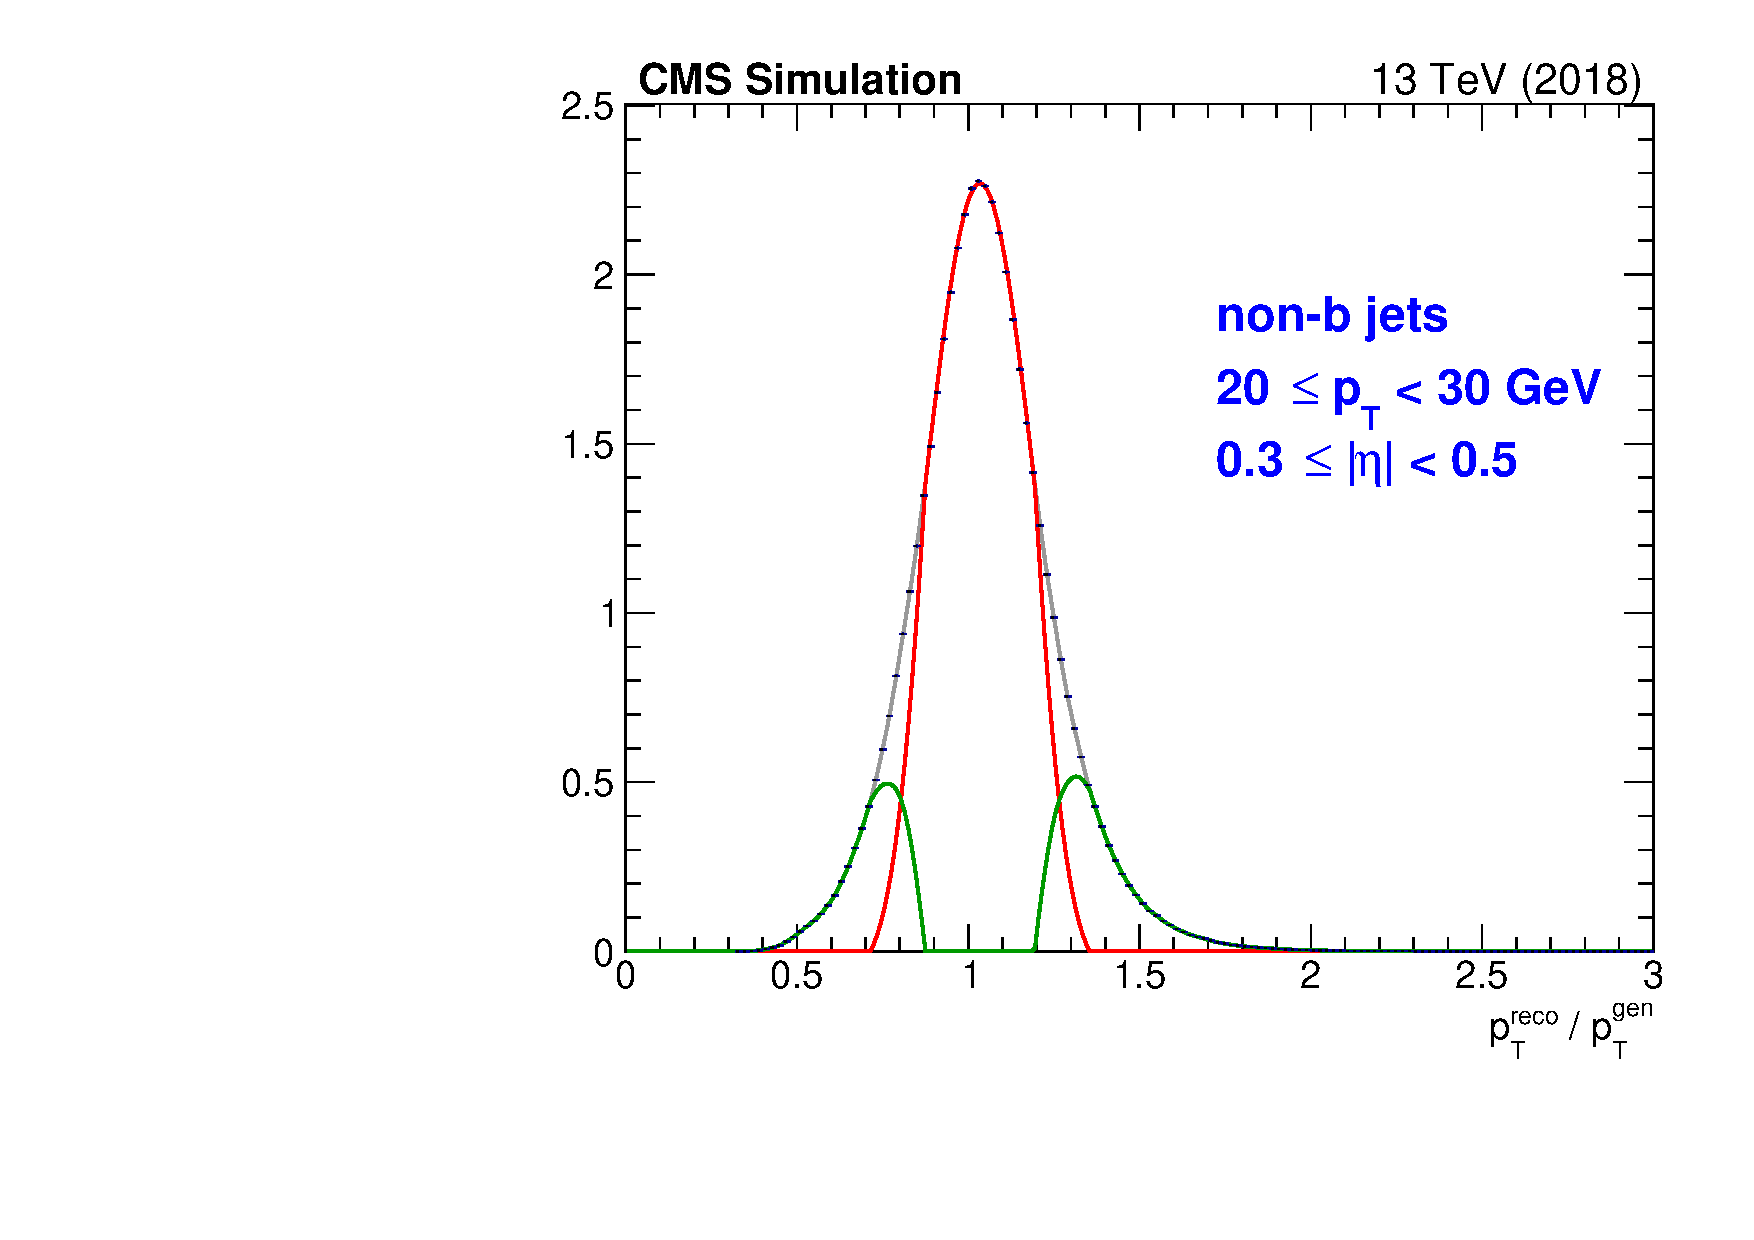
\includegraphics[width=0.45\textwidth]{figs/jetmet/pt01_eta01_nonbjets_lin.pdf}
    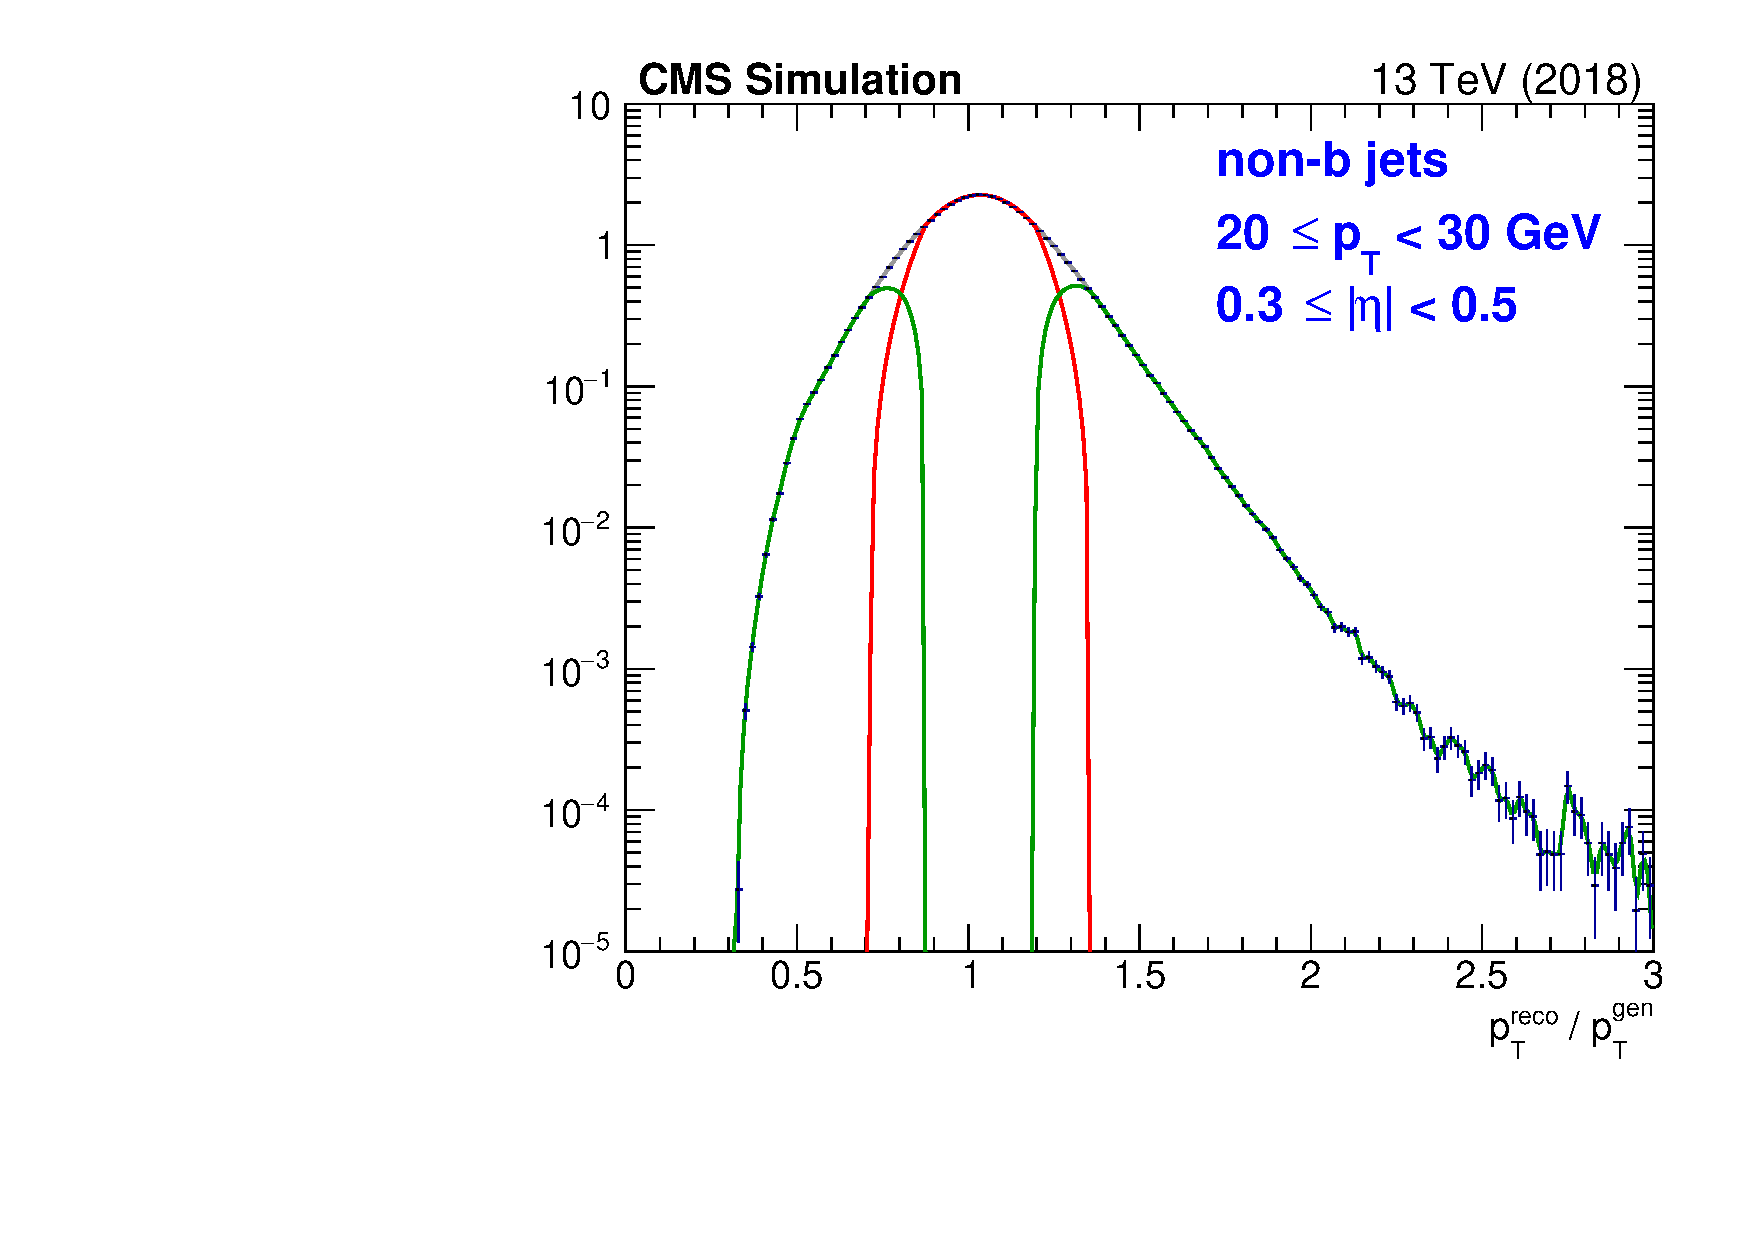
\includegraphics[width=0.45\textwidth]{figs/jetmet/pt01_eta01_nonbjets_log.pdf} \\
    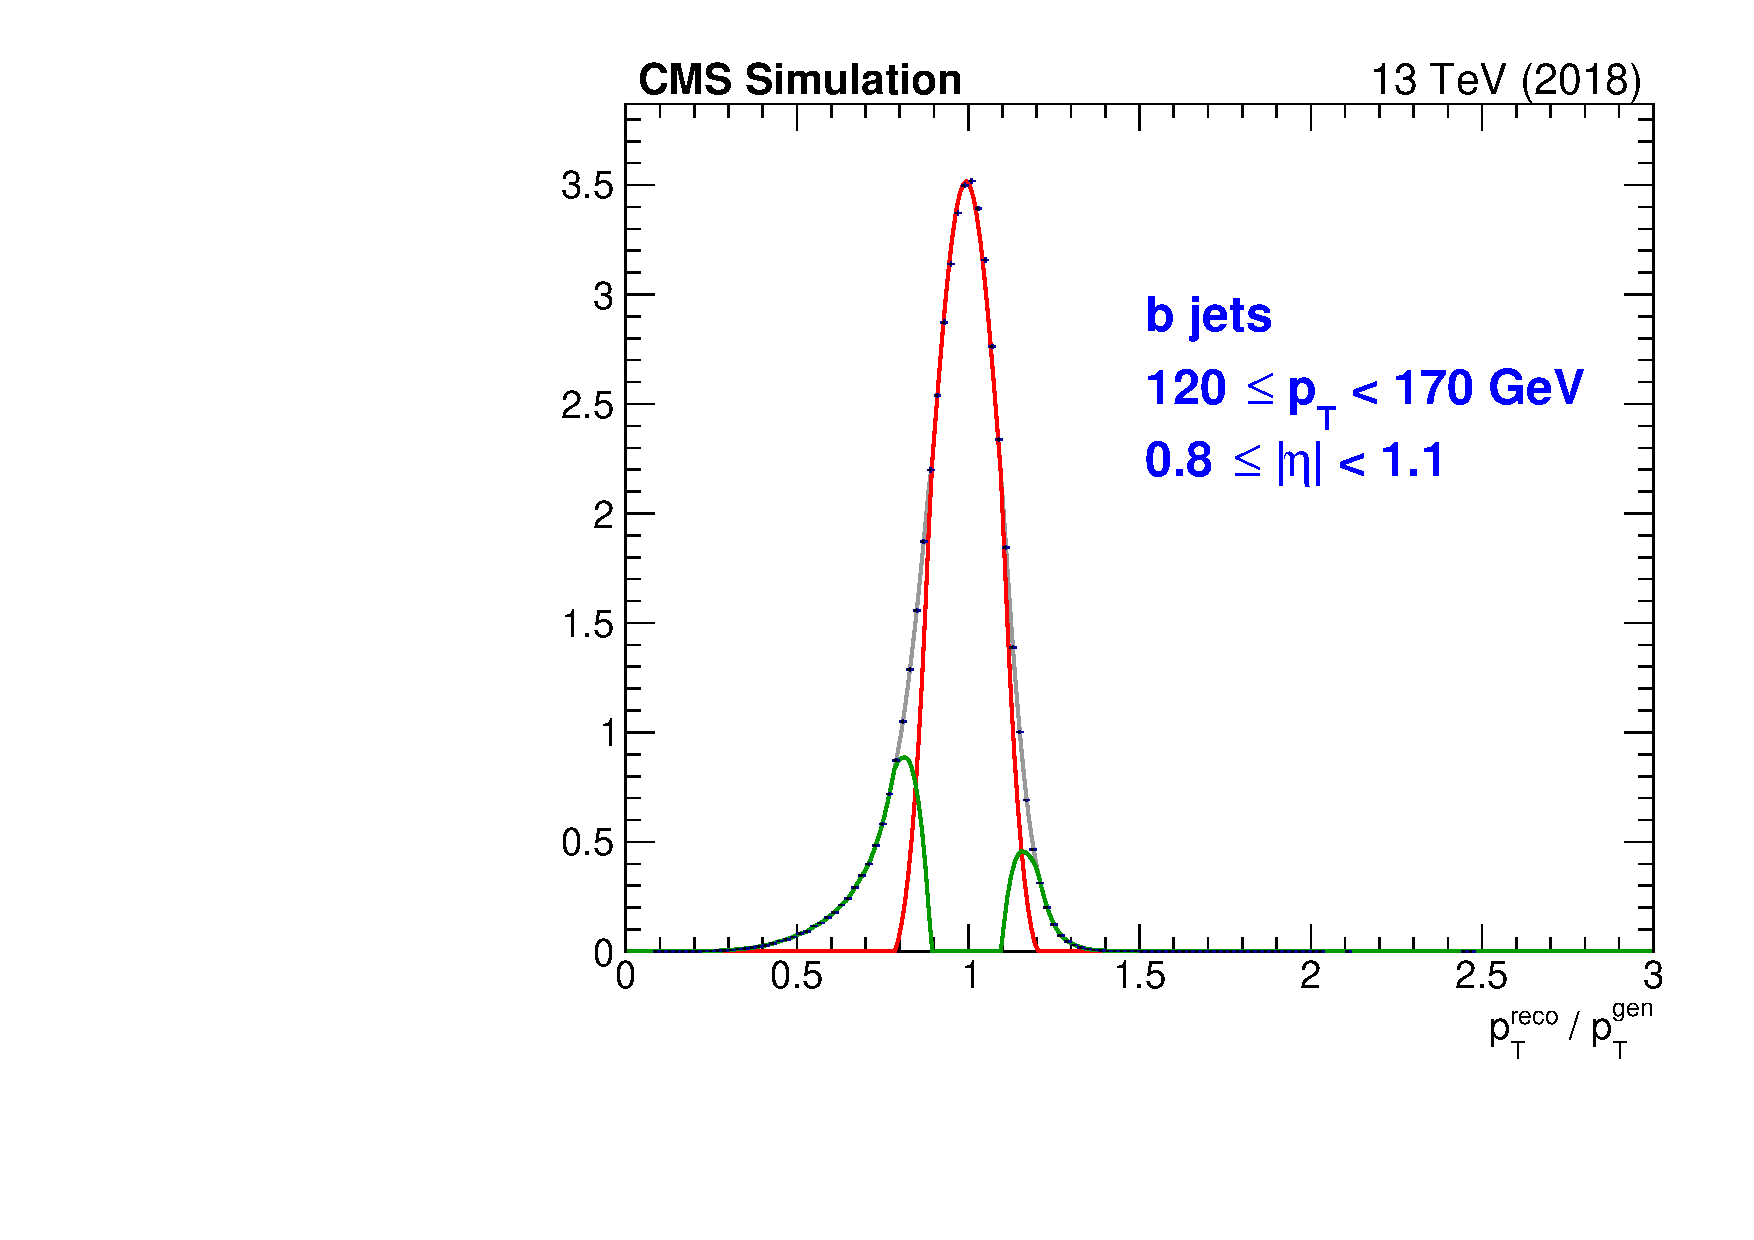
\includegraphics[width=0.45\textwidth]{figs/jetmet/pt05_eta03_bjets_lin.pdf}
    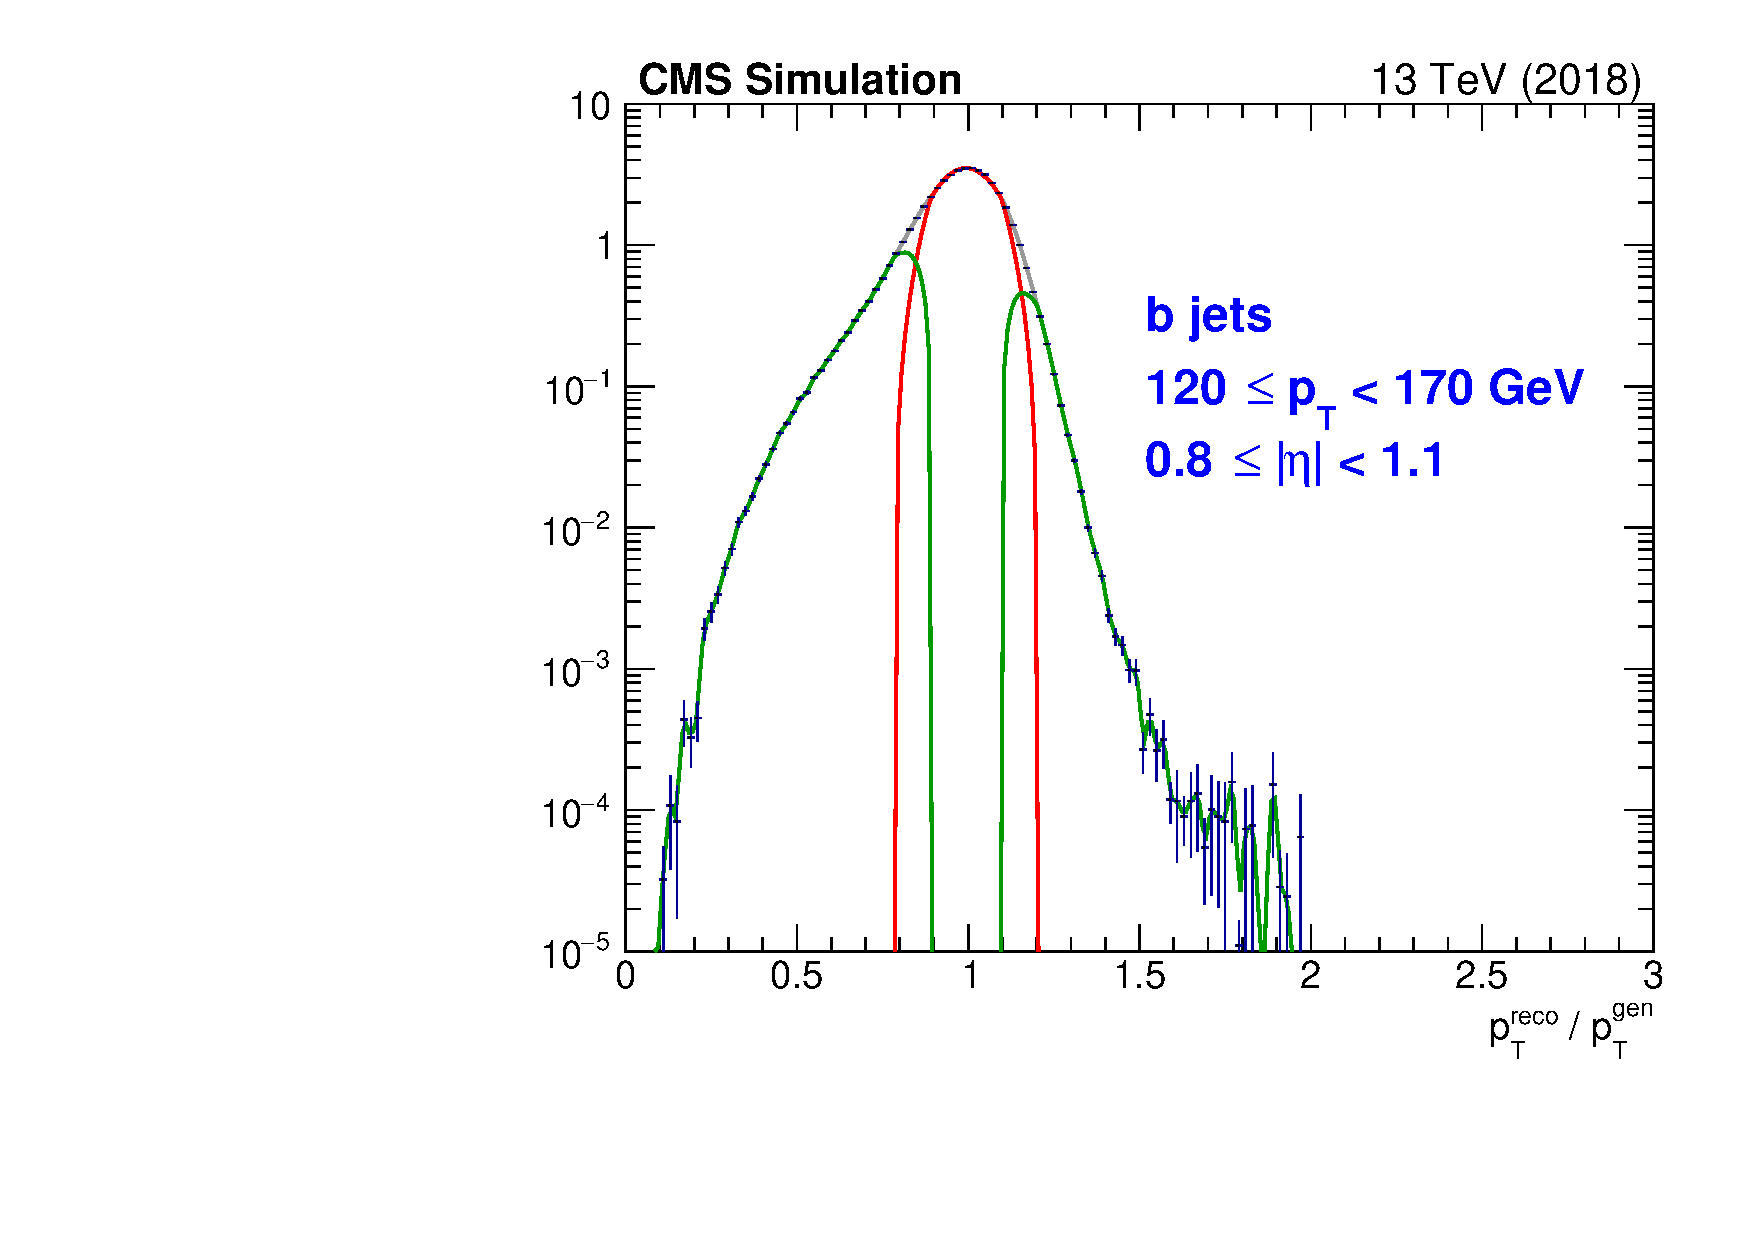
\includegraphics[width=0.45\textwidth]{figs/jetmet/pt05_eta03_bjets_log.pdf} \\
    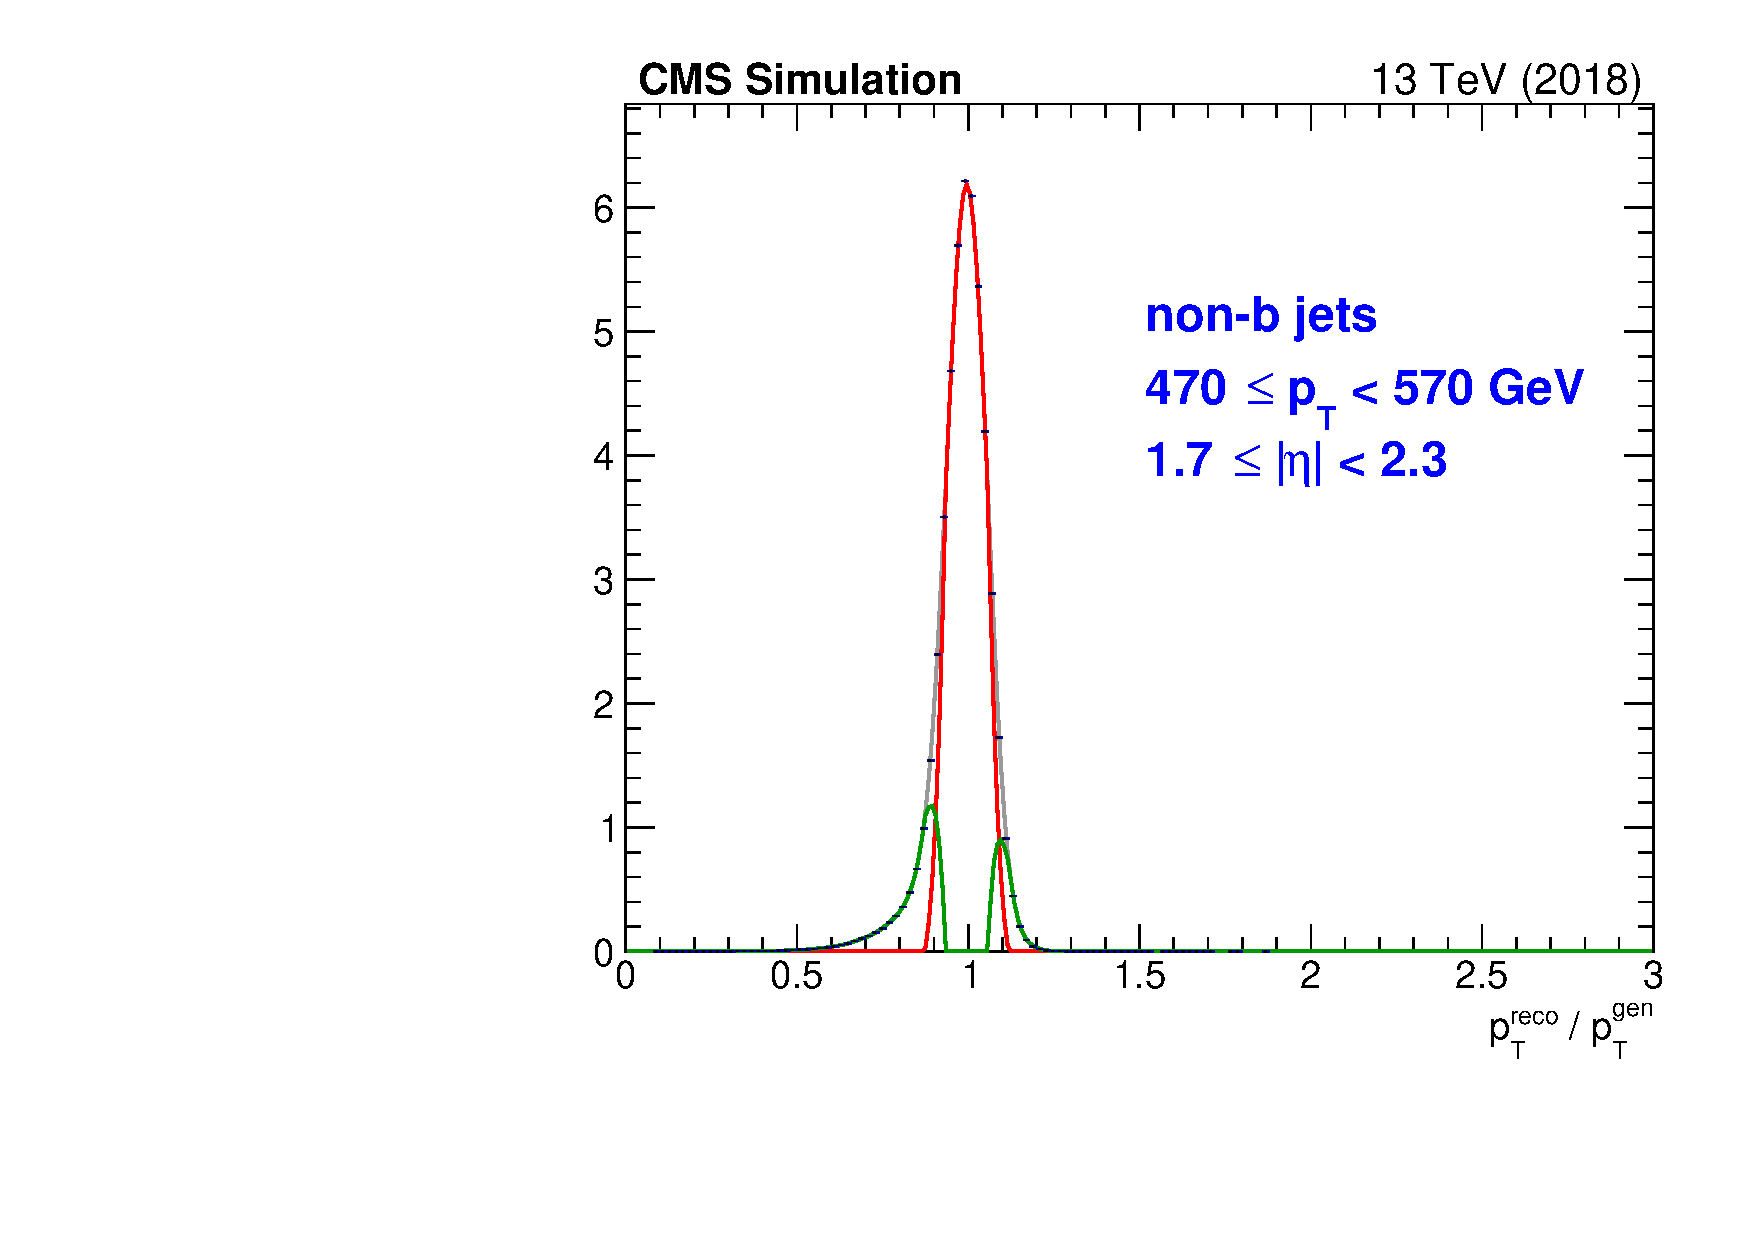
\includegraphics[width=0.45\textwidth]{figs/jetmet/pt10_eta06_nonbjets_lin.pdf}
    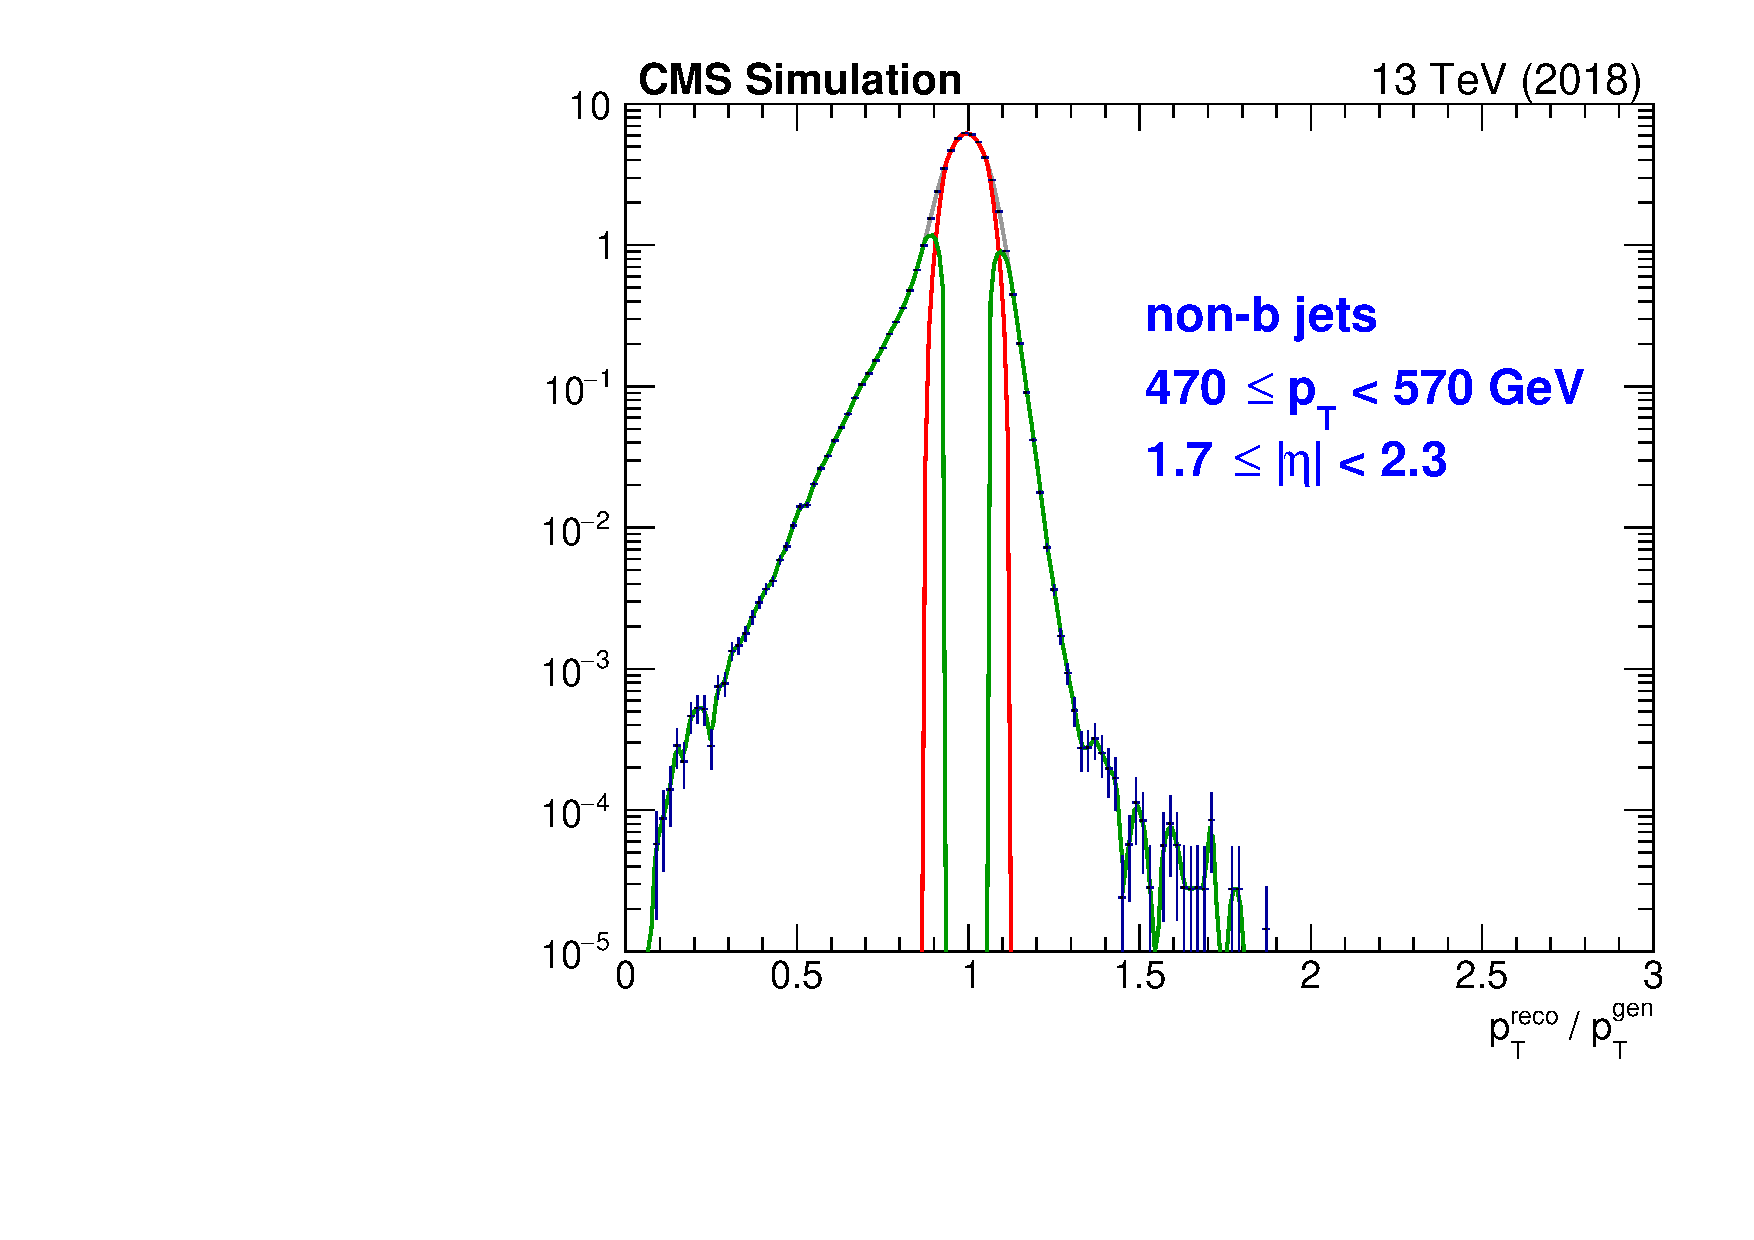
\includegraphics[width=0.45\textwidth]{figs/jetmet/pt10_eta06_nonbjets_log.pdf} \\
    \caption{A selection of three example jet response templates for various \pt/$\eta$/b-jet bins, shown in linear (left) and log (right) scales.
    The dark blue points are the raw templates. The red curves are the fitted gaussian ``cores'' of the templates, and the green
    curves are the ``tails'', as described in Section~\ref{sec:jrt_fits}.
           }
    \label{fig:jrt_examples}
  \end{center}
\end{figure}

\begin{figure}[htbp]
  \begin{center}
    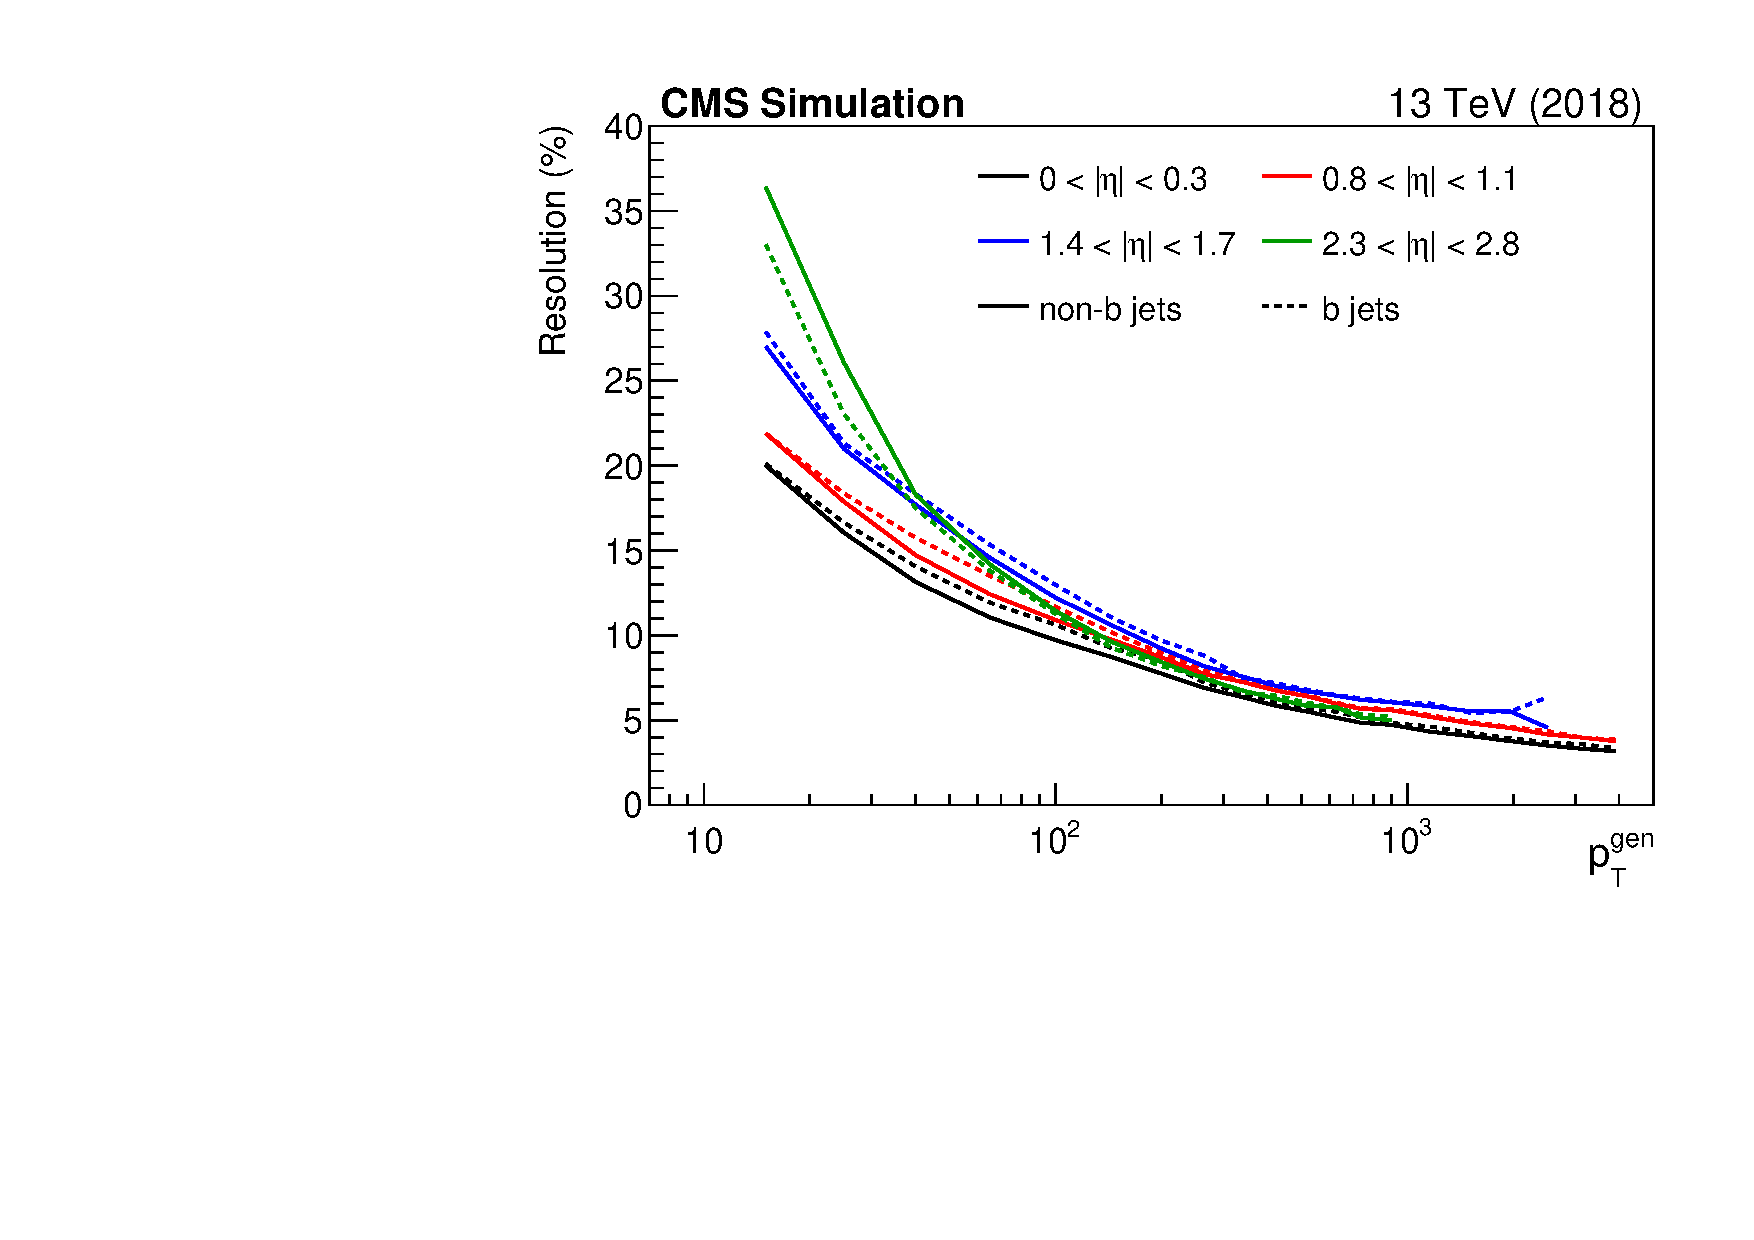
\includegraphics[width=0.49\textwidth]{figs/jetmet/resolution_vs_pt.pdf}
    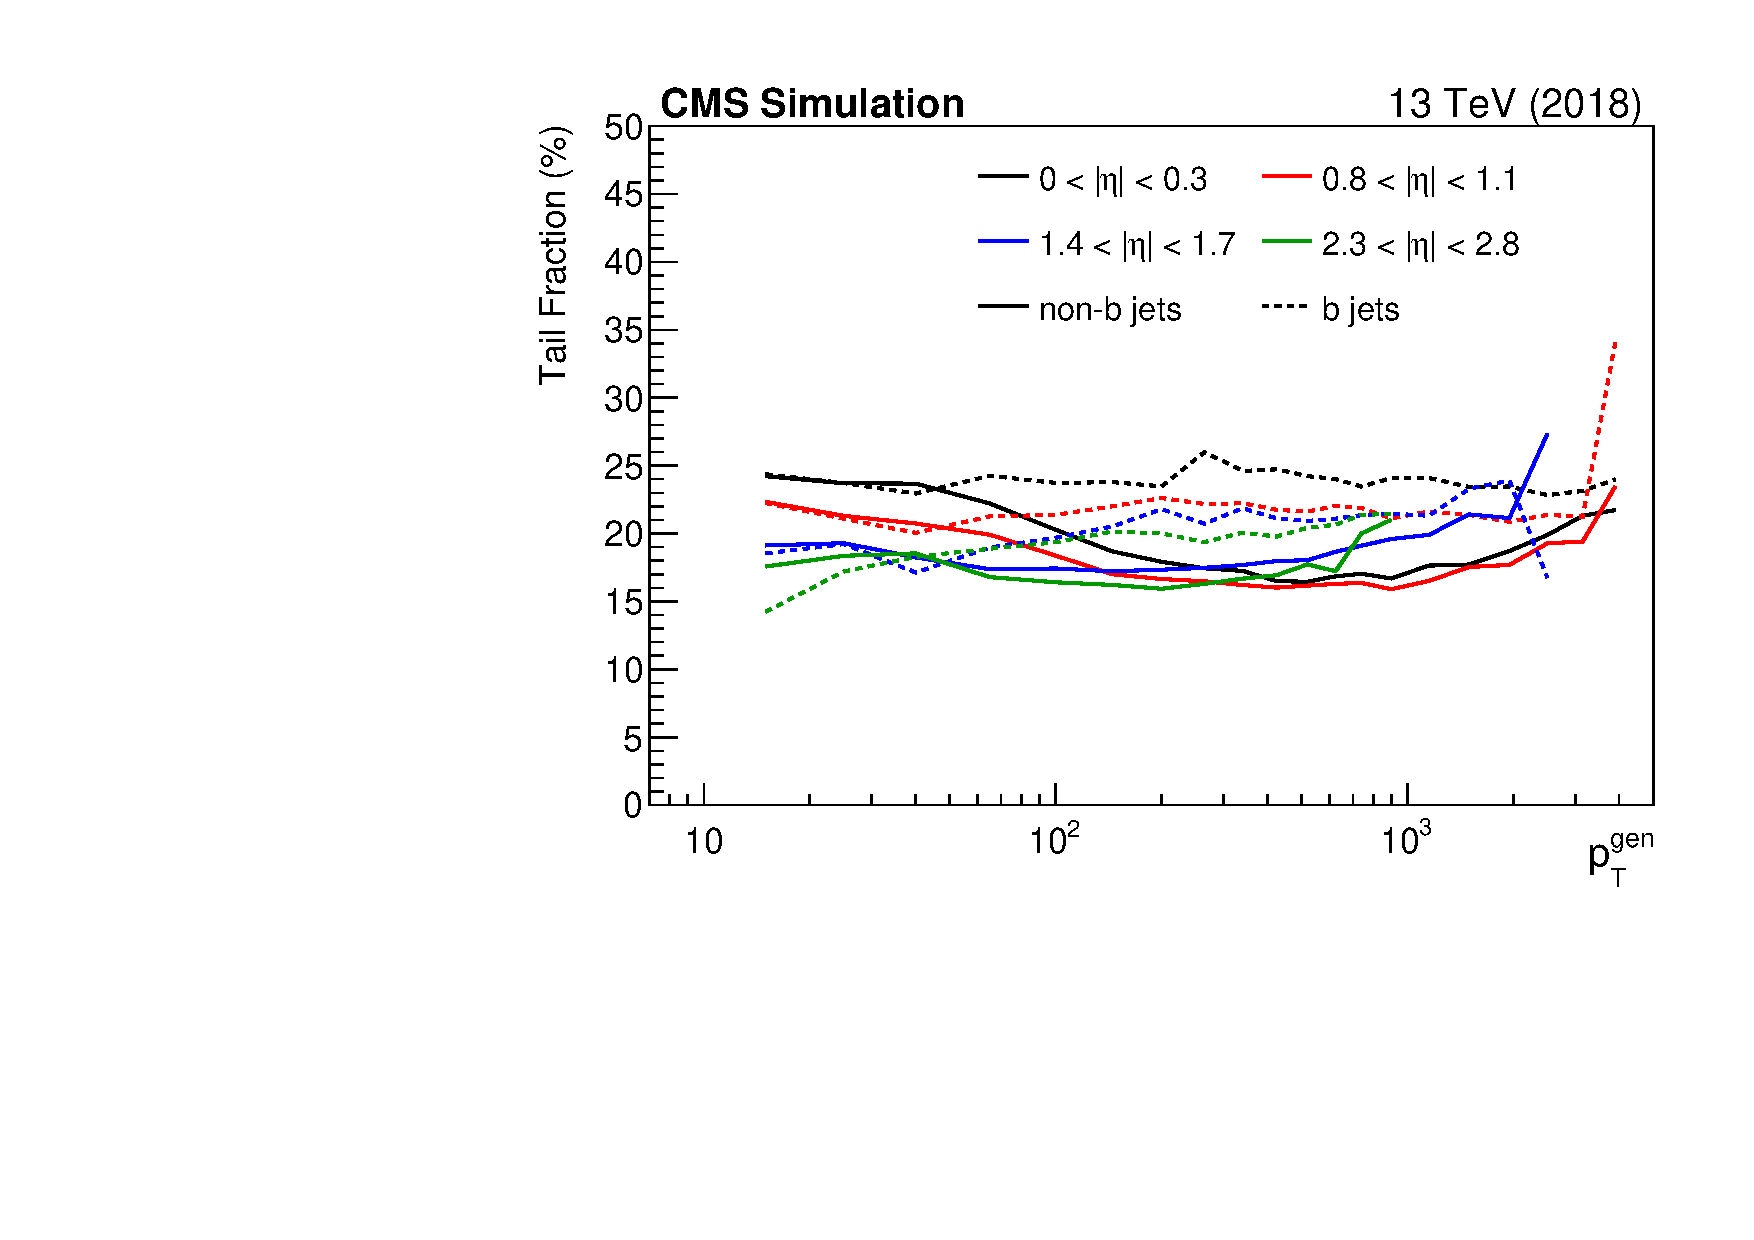
\includegraphics[width=0.49\textwidth]{figs/jetmet/tailfrac_vs_pt.pdf}
    \caption{(left) Jet energy resolution (defined as the width of the fitted gaussian core) as a function of generator-level jet \pt, as measured in Autumn18 MC. 
    Resolution improves as jet \pt increases, and generally degrades as $\eta$ increases.
    (right) The fraction of the jet response function that resides in the fitted tails (as opposed to the gaussian core) as a function of generator-level jet \pt, 
    as measured in Autumn 18 MC. The main feature to notice is that at intermediate \pt,  b jets have a higher probability to be in the tail. This is due to the presence
    of neutrinos from heavy-flavor decay in the jet, which cause the jet energy to be undermeasured and hence enhance the left tail of the templates. At low \pt, the
    tails are driven by other effects so differences between b and non-b jets are not visible.
    }
    \label{fig:jrt_res_pt}
  \end{center}
\end{figure}


\subsection{Gen/reco jet matching}
\label{sec:jrt_matching}

The process for matching gen and reco jets in order to derive jet response templates begins with QCD Monte Carlo,
in which both the generator-level and reconstructed particles have been clustered into jets.
It is important to use gen jets that include neutrinos, as we are interested in modeling jet mismeasurement due
to energy carried away by neutrinos such. Reco jet energies are fully corrected with the same jet energy corrections
as used in the main analysis. Gen jet flavor is determined by identifying the flavor of 
hadrons within the jet cone. Once this is all done, all reco and gen jets with $\pt>10$ GeV are selected and saved.

After selecting the jets, gen and reco jets are matched and JRTs are constructed by 
filling histograms with $\pt^\text{reco}/\pt^\text{gen}$.
The algorithm for matching is outlined here; the reasoning for and effect of various steps are described following.
\begin{enumerate}
\item Skip events that fail any of the MET filters used in the main analysis
\item Find all ``tight pairs'' of reco/gen jets that have $\Delta R$(reco, gen) $<0.3$
\item Find all ``loose pairs'' of reco/gen jets that have $\Delta R$(reco, gen) $<0.5$
\item Identify the reco jets and gen jets that are in more than one loose pair
\item Throw away any tight pairs that contain a jet identified in the previous step
\item Throw away pairs where in which the reco jet is within one of the manually-identified calorimeter holes
\item Throw away pairs where in which the reco jet fails tight jet ID
\item Throw away pairs where in which the reco jet fails loose pileup jet ID
\item For all remaining tight pairs, identify the correct \pt/$\eta$-binned histograms and fill:
  \begin{itemize}
    \item b jet histogram with weight \\
    \hphantom{1 cm}$w_\text{b}=\varepsilon_\text{b-tag}$(\pt, $\eta$, gen flavor) $\times$ $SF_\text{b-tag}$(\pt, $\eta$, gen flavor),
    \item non-b jet histogram with weight \\
    \hphantom{1 cm}$w_\text{non-b} = 1-w_\text{b}$,
  \end{itemize}
  where $\varepsilon_\text{b-tag}$ is the efficiency for tagging a particular flavor of gen jet, as measured in MC, and $SF_\text{b-tag}$ is 
  the CMS-derived scale factor to correct this efficiency for known differences between data and MC.
\end{enumerate}

Step 1 rejects entire events that fail one of the MET filters applied in the main analysis.
These guard against certain kinds of mis-reconstruction that can enhance the tails of the
jet response functions. Most notably, the EcalDeadCellTriggerPrimitive and HBHENoise filters
reject events where there is energy in calorimeter regions known to be down/noisy (leading to 
fake energy, and enhancement of the right tails), and the BadChargedCandidate and BadPFMuon
filters reject events containing badly reconstructed high-\pt tracks (which also enhance
the right tails). Since we reject these events in the main analysis, we also reject
jets from such events here to avoid false tails in the templates 
(see Fig.~\ref{fig:jrt_matching_effect} (right) for an example of the effect on a template)

Steps 2 through 5 identify pairs of gen and reco jets with $\Delta R<0.3$, but with the crucial caviat that 
\emph{there are no additional matches within} $\Delta R<0.5$. This protects against one of the largest fake sources
of tails in the measured templates: the ``splitting'' of gen and/or reco jets. This can happen in three distinct ways:
\begin{itemize}
  \item A single gen jet is reconstructed as multiple reco jets, and gets matched to one. 
  This enhances the left tail of the templates, as the matched reco jet only has a fraction of the energy.
  \item Multiple gen jets are reconstructed as a single reco jet. This enhances the right tail of the 
  templates, as the matched gen jet only has a fraction of the energy.
  \item There are multiple nearby gen and reco jets, but energy/particles are distributed differently 
  among the gen jets compared to reco. This enhances both tails, depending on how the energy distribution
  and matching happens.
\end{itemize}
Requiring that there are no secondary nearby gen (reco) jets within $\Delta R<0.5$ of the reco (gen) jet protects against these scenarios.
The effect on a sample template is shown in Fig.~\ref{fig:jrt_matching_effect}. 
The reduction in the tails after applying this cut is seen to be quite large.

\begin{figure}[htbp]
  \begin{center}
    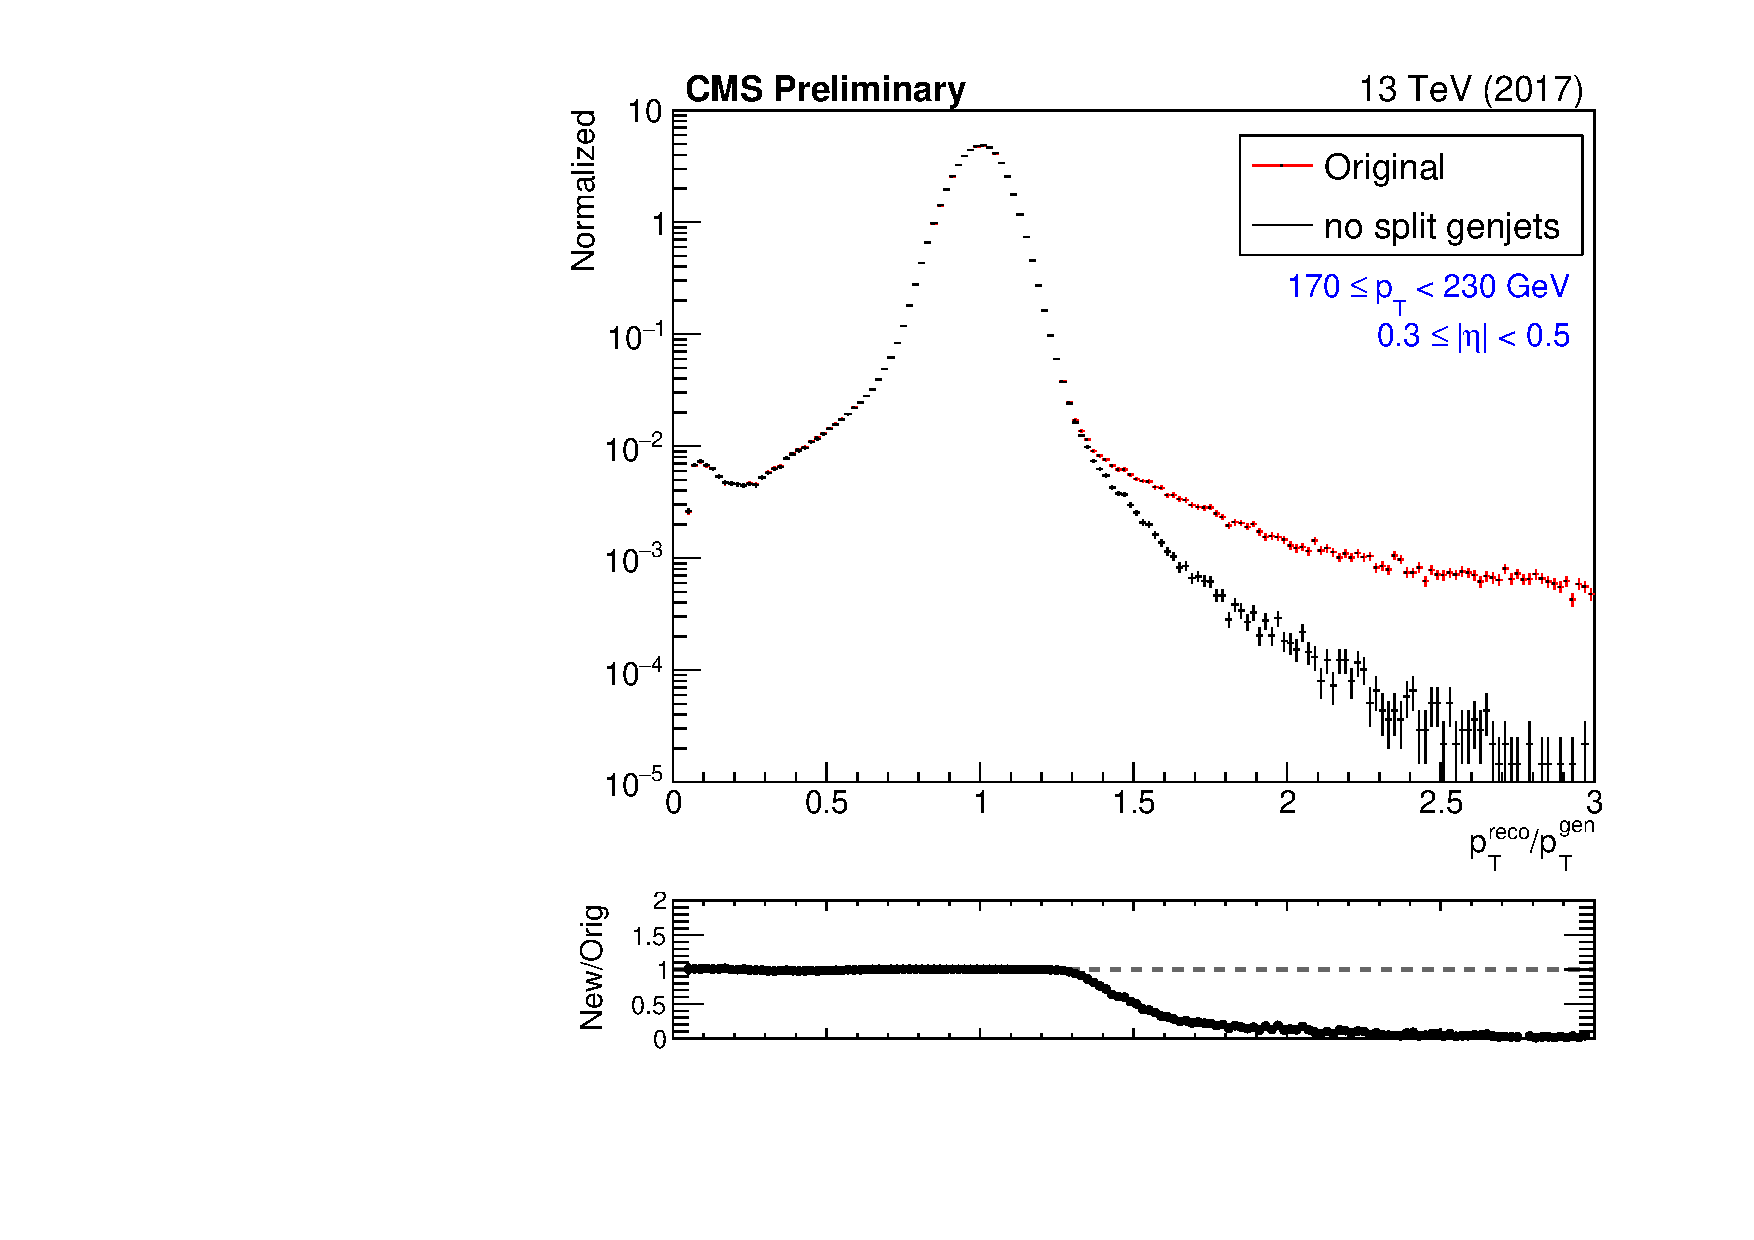
\includegraphics[width=0.325\textwidth]{figs/jetmet/compare_noSplitGen.pdf}
    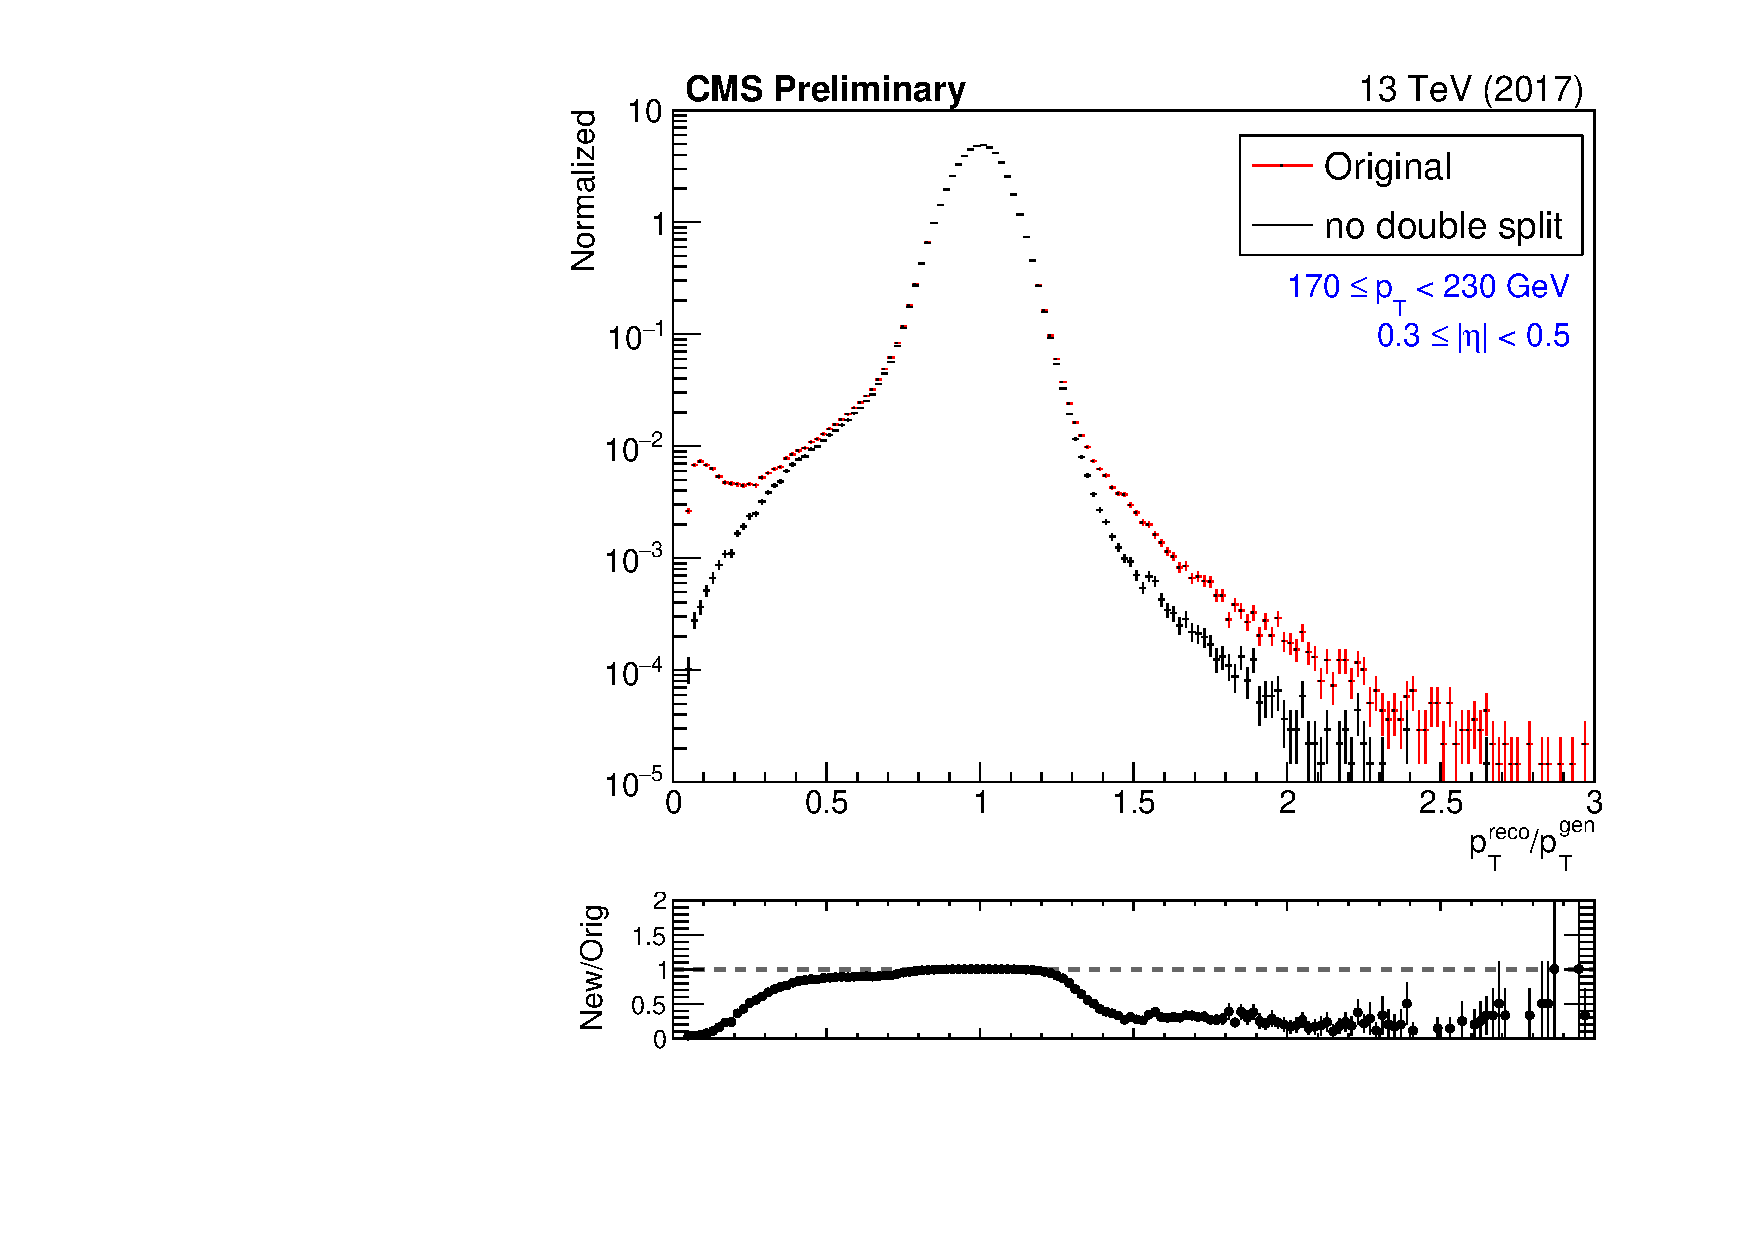
\includegraphics[width=0.325\textwidth]{figs/jetmet/compare_noDoubleSplit.pdf}
    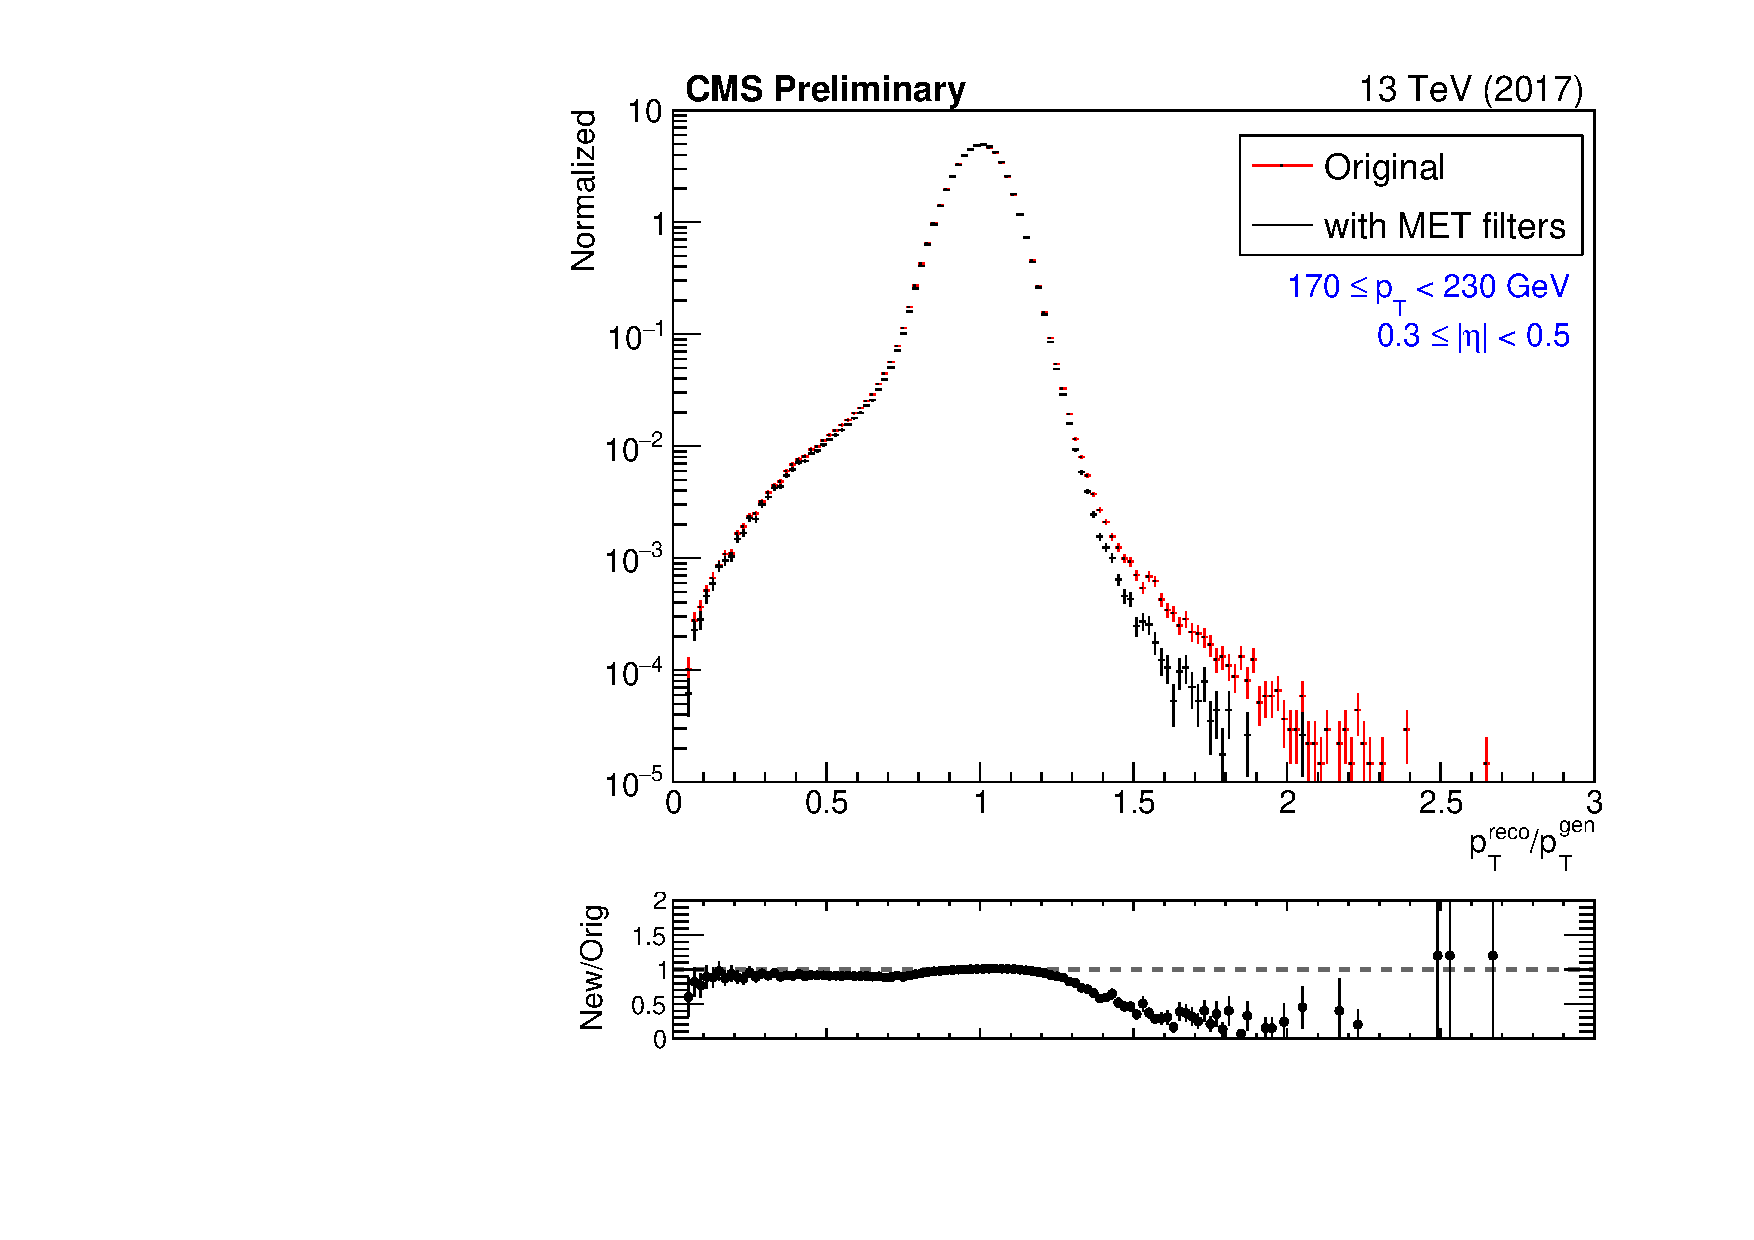
\includegraphics[width=0.325\textwidth]{figs/jetmet/compare_metFilters.pdf}
    \caption{The effect of various cuts applied during the matching on an example template (non-b jet, $170 \leq \pt < 230$ GeV, $0.3 \leq |\eta| < 0.5$).
    (left) Requiring \emph{exactly} 1 gen jet within $\text{dR}<0.3$ of a reco jet, instead of at least one. This removes ``split'' gen jets.
    (center) Requiring that there are no secondary nearby gen (reco) jets within $\text{dR}<0.5$ of the reco (gen) jet. This protects
    against splitting in both directions, so reduces both tails.
    (right) Applying MET filters and rejecting jets from events that fail. This removes bad reconstructions (e.g. fake high-\pt track) and
    primarily reduces the right tail.
    }
    \label{fig:jrt_matching_effect}
  \end{center}
\end{figure}

Step 6 throws away pairs involving a reco jet in one of a number of manually-identified ``dead'' spots in the detector.
When plotting an $\eta-\phi$ map of the jets with small ($<$0.5) $\pt^\text{reco}/\pt^\text{gen}$ values,
we observe a number of ``hot-spots'', corresponding to calorimeter regions that are dead or off in the simulation.
These do not generally correspond to real effects in the data, and lead to artificially large left tails in the templates.
We identify these regions (separately for each year) and remove any jet pairs that contain a reco jet in one of these regions.
Fig.~\ref{fig:jrt_ecalDeadCell} shows these cells highlighted for 2017 simulation on the left, and
the effect on an example template on the right.

\begin{figure}[htbp]
  \begin{center}
    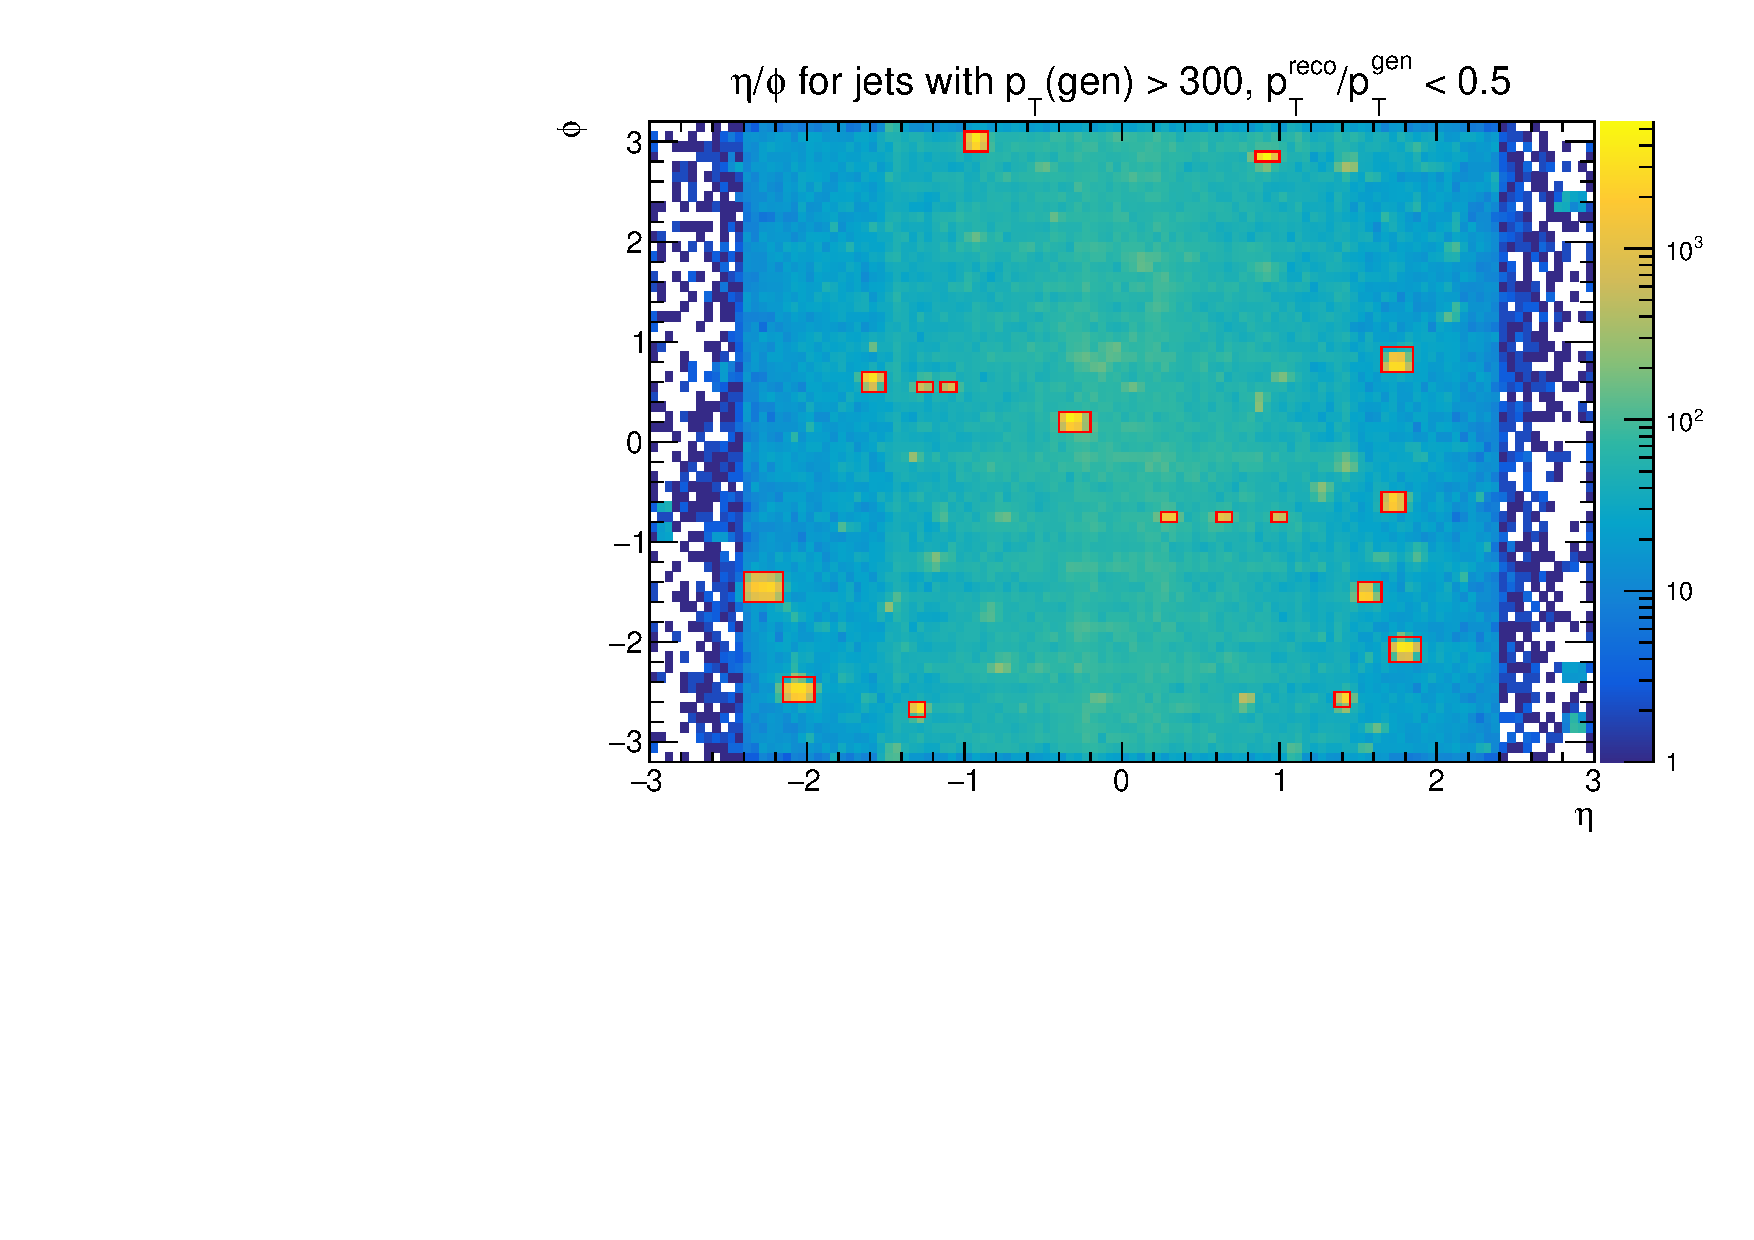
\includegraphics[width=0.54\textwidth]{figs/jetmet/ecalDeadCells.pdf}
    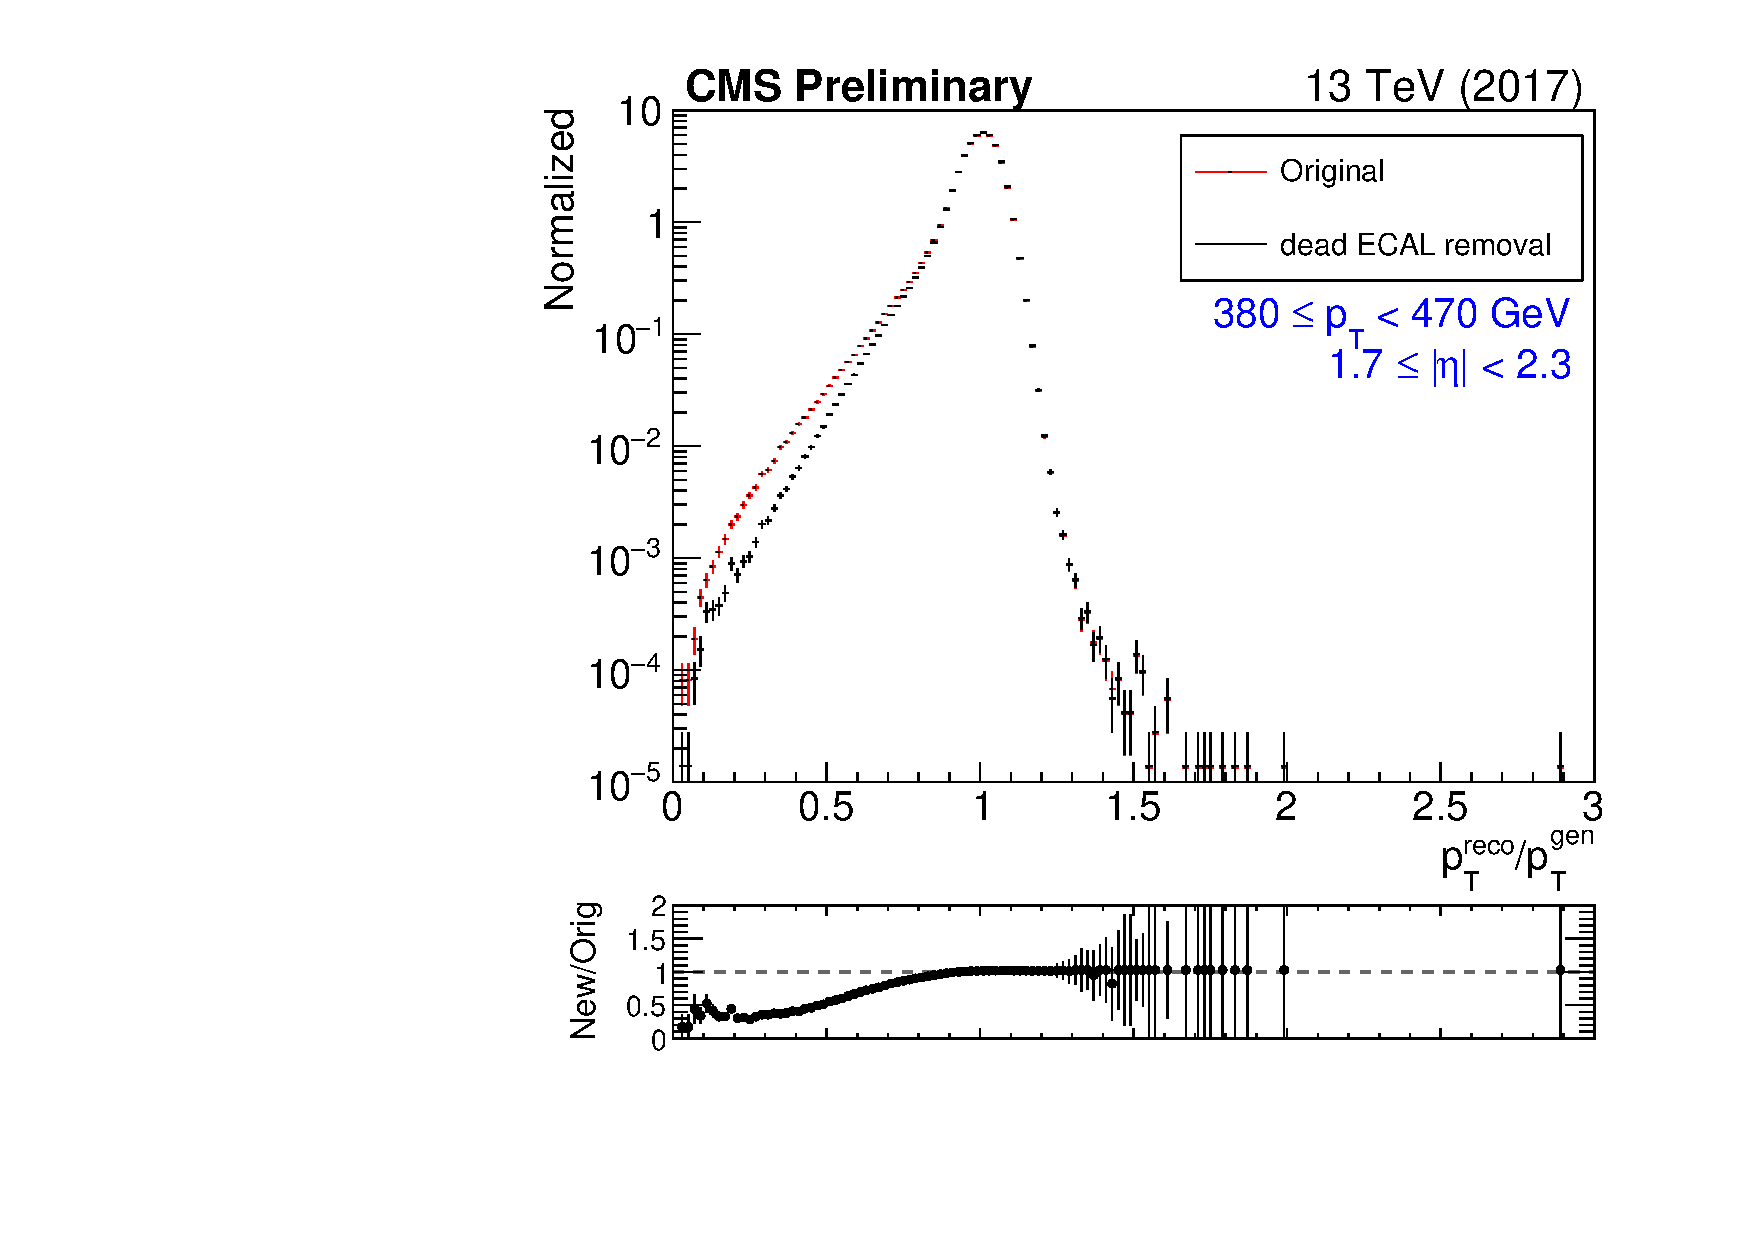
\includegraphics[width=0.45\textwidth]{figs/jetmet/compare_ecalDeadCell.pdf}
    \caption{(left) an $\eta-\phi$ map for jet pairs with $\pt^\text{gen}> 300$ GeV and
    $\pt^\text{reco}/\pt^\text{gen} < 0.5$ from 2017 simulation. Identified hot-spots
    are outlined in red. Pairs with reco jets in these regions are not used.
    (right) The effect of this removal on an example template. Relatively large reductions
    in the left tail are seen for templates containing affected regions.
    }
    \label{fig:jrt_ecalDeadCell}
  \end{center}
\end{figure}

Step 7 rejects pairs in which the reco jet fails tight jet ID.
In the main analysis, we reject the entire event if any jet with $\pt>30$ GeV
fails this ID. We apply the same ID here to avoid including these jets in 
the templates. It is found to have minimal effect, except for very high eta ($|\eta|>4.0$).

Step 8 rejects jets that fail loose pileup jet ID~\cite{JME_pileup_id}. In the rebalancing and smearing steps,
jets with $\pt<100$ GeV that fail this pileup ID are left untouched (i.e., not included
in the rebalancing and not smeared), in order to avoid trying to balance an event
against a pileup jet. Since we do not use them in the rebalancing and smearing, 
we do not want to include them in the templates.
Vetoing jets that fail pileup ID has a fairly significant effect on the tails.
At higher \pt, we see a reduction in the left tail from gen jets that were
mis-matched to a low-\pt pileup jet. At lower \pt, we see a reduction in both tails
(see Fig.~\ref{fig:jrt_jetid}).

\begin{figure}[htbp]
  \begin{center}
    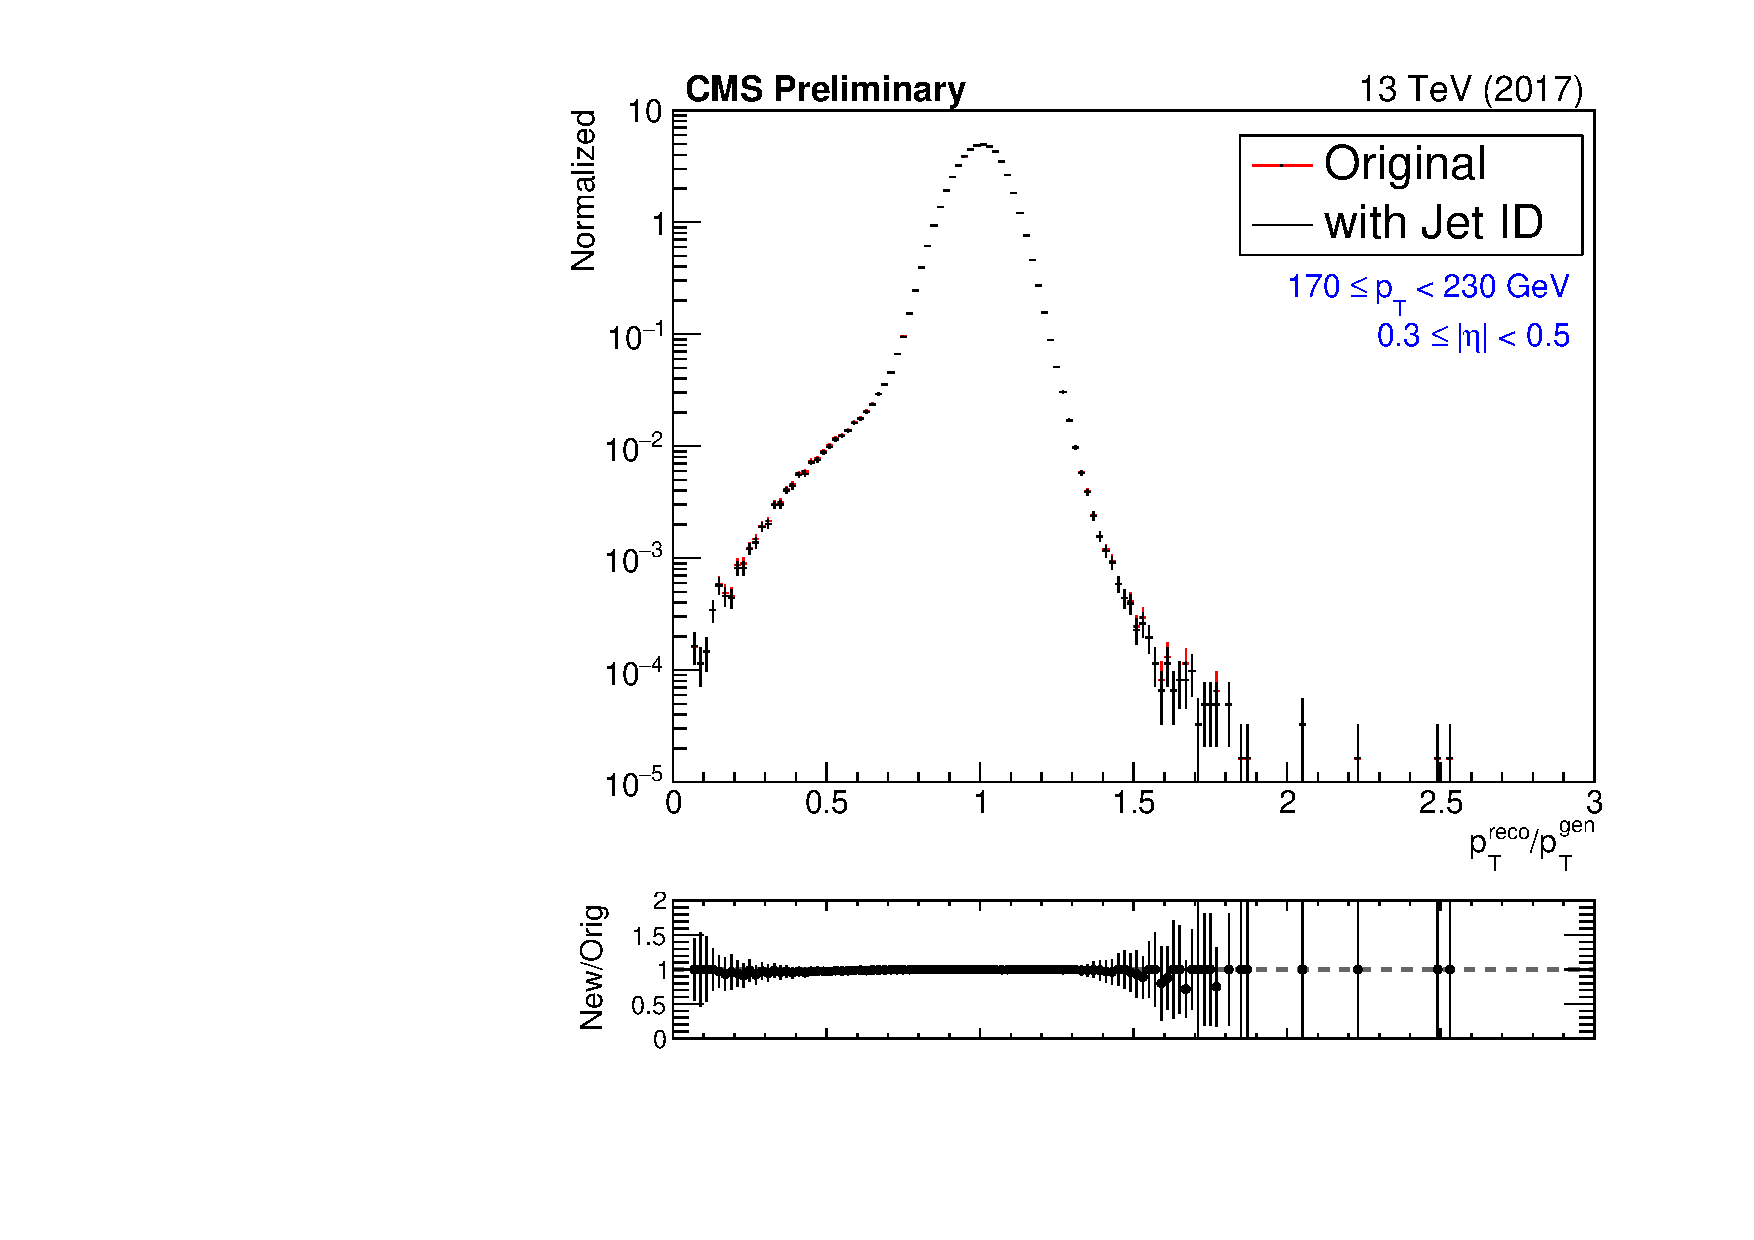
\includegraphics[width=0.325\textwidth]{figs/jetmet/compare_jetID.pdf}
    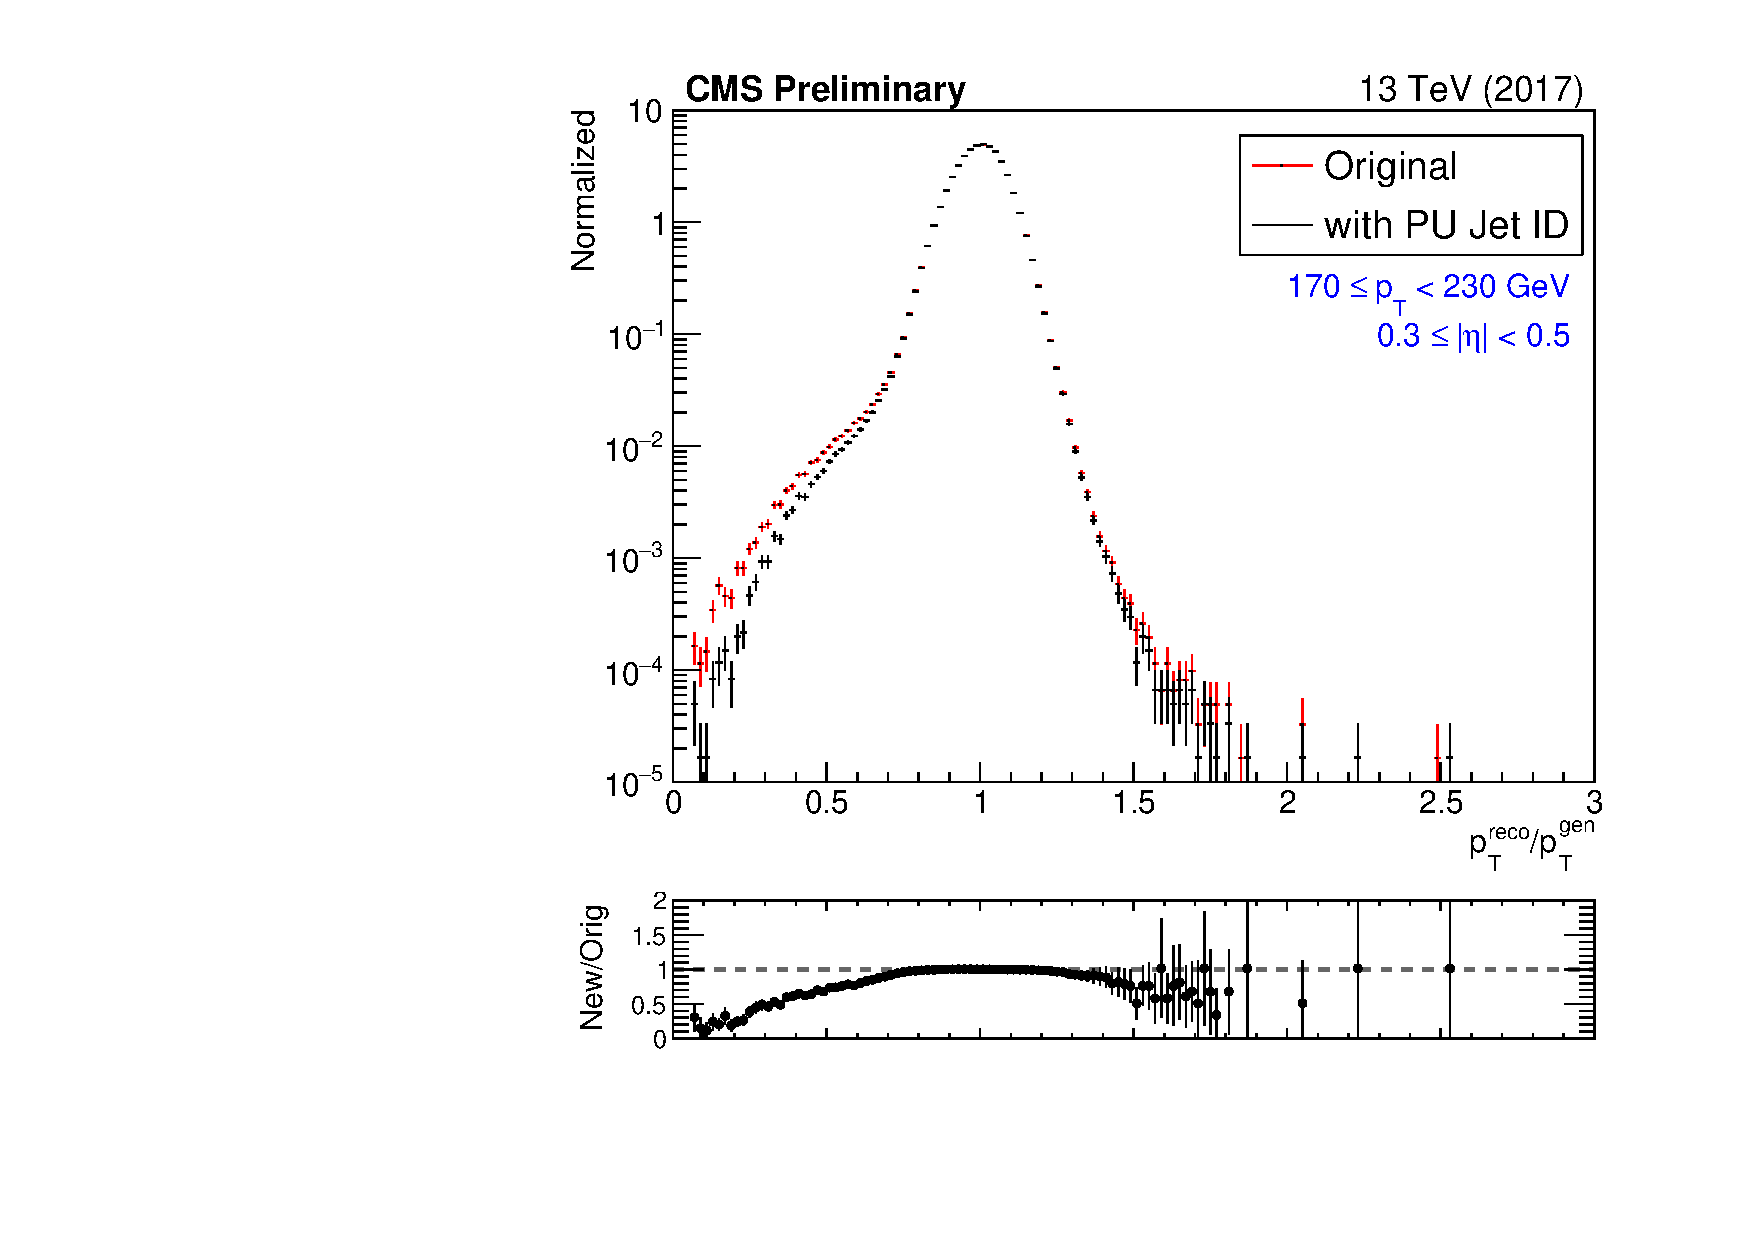
\includegraphics[width=0.325\textwidth]{figs/jetmet/compare_puJetID_highPt.pdf}
    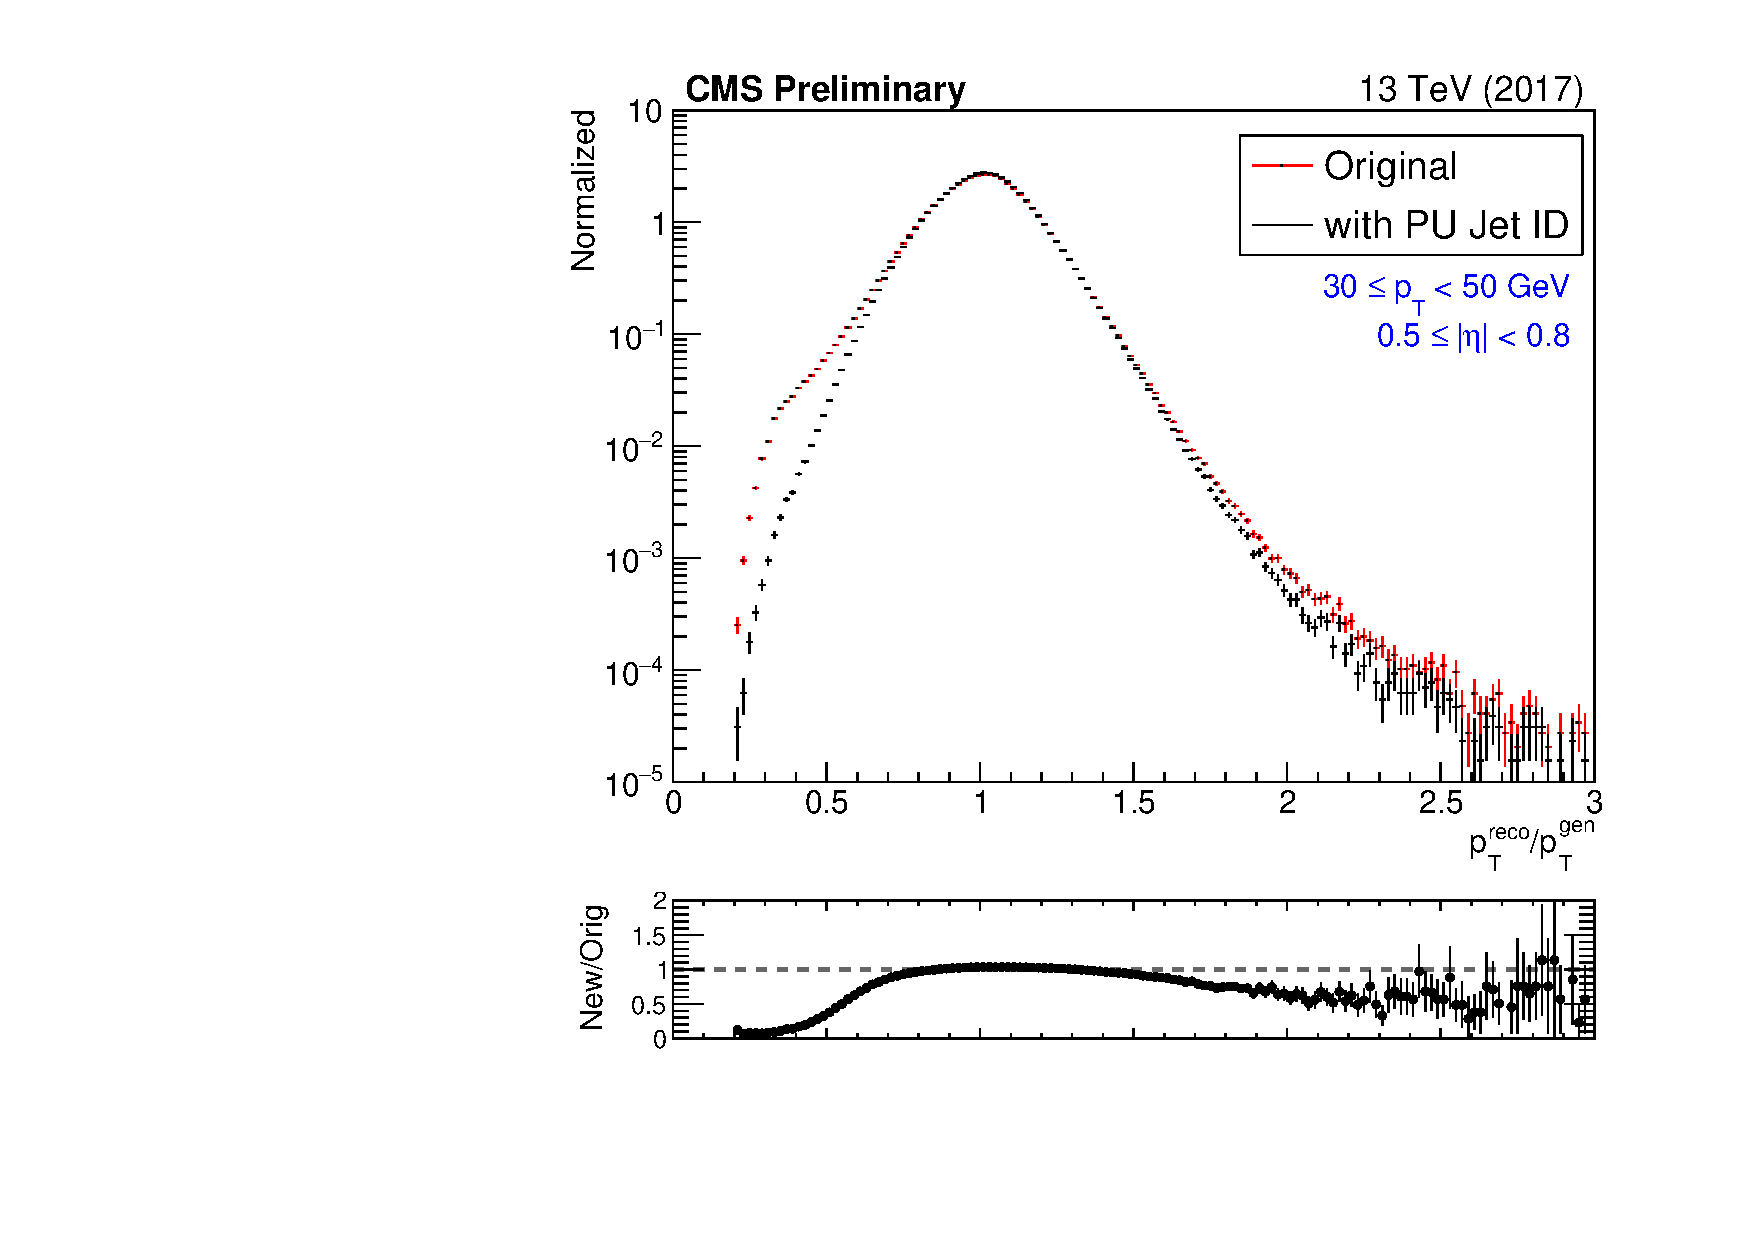
\includegraphics[width=0.325\textwidth]{figs/jetmet/compare_puJetID_lowPt.pdf}
    \caption{(left) and (center) show the effect of applying tight jet ID and loose pileup jet ID, respectively,
    to the same template as in Fig.~\ref{fig:jrt_matching_effect}. Jet ID has negligible effect,
    while the pileup jet ID leads to a reduction in the left tail.
    (right) The effect of pileup jet ID on a lower \pt template ($30\leq\pt<50$ GeV). Here we observe
    a reduction in both tails.
    }
    \label{fig:jrt_jetid}
  \end{center}
\end{figure}

In the final step, we have identified jet pairs and need to fill histograms. The only thing left to decide
is how to fill the b and non-b jet templates. There are three options that have all been tried:
\begin{enumerate}
  \item Fill only a single histogram, based on the gen jet flavor (found by identifying flavor of hadrons within jet).
  \item Fill only a single histogram, based on whether the reco jet is medium b-tagged.
  \item Fill both histograms, with weights given by the probability of tagging that jet as a b jet (corrected with data/MC scale factors).
\end{enumerate}

We evaluate each method empirically by observing the agreement in \nbtags in QCD-enriched control regions after applying
the full Rebalance and Smear method described in Chapter~\ref{chap:qcd}. It is found that (2) slightly improves on (1), and (3) is quite a bit better than both.
An example of the effect is shown in Fig.~\ref{fig:jrt_nb}.

\begin{figure}[htbp]
  \begin{center}
    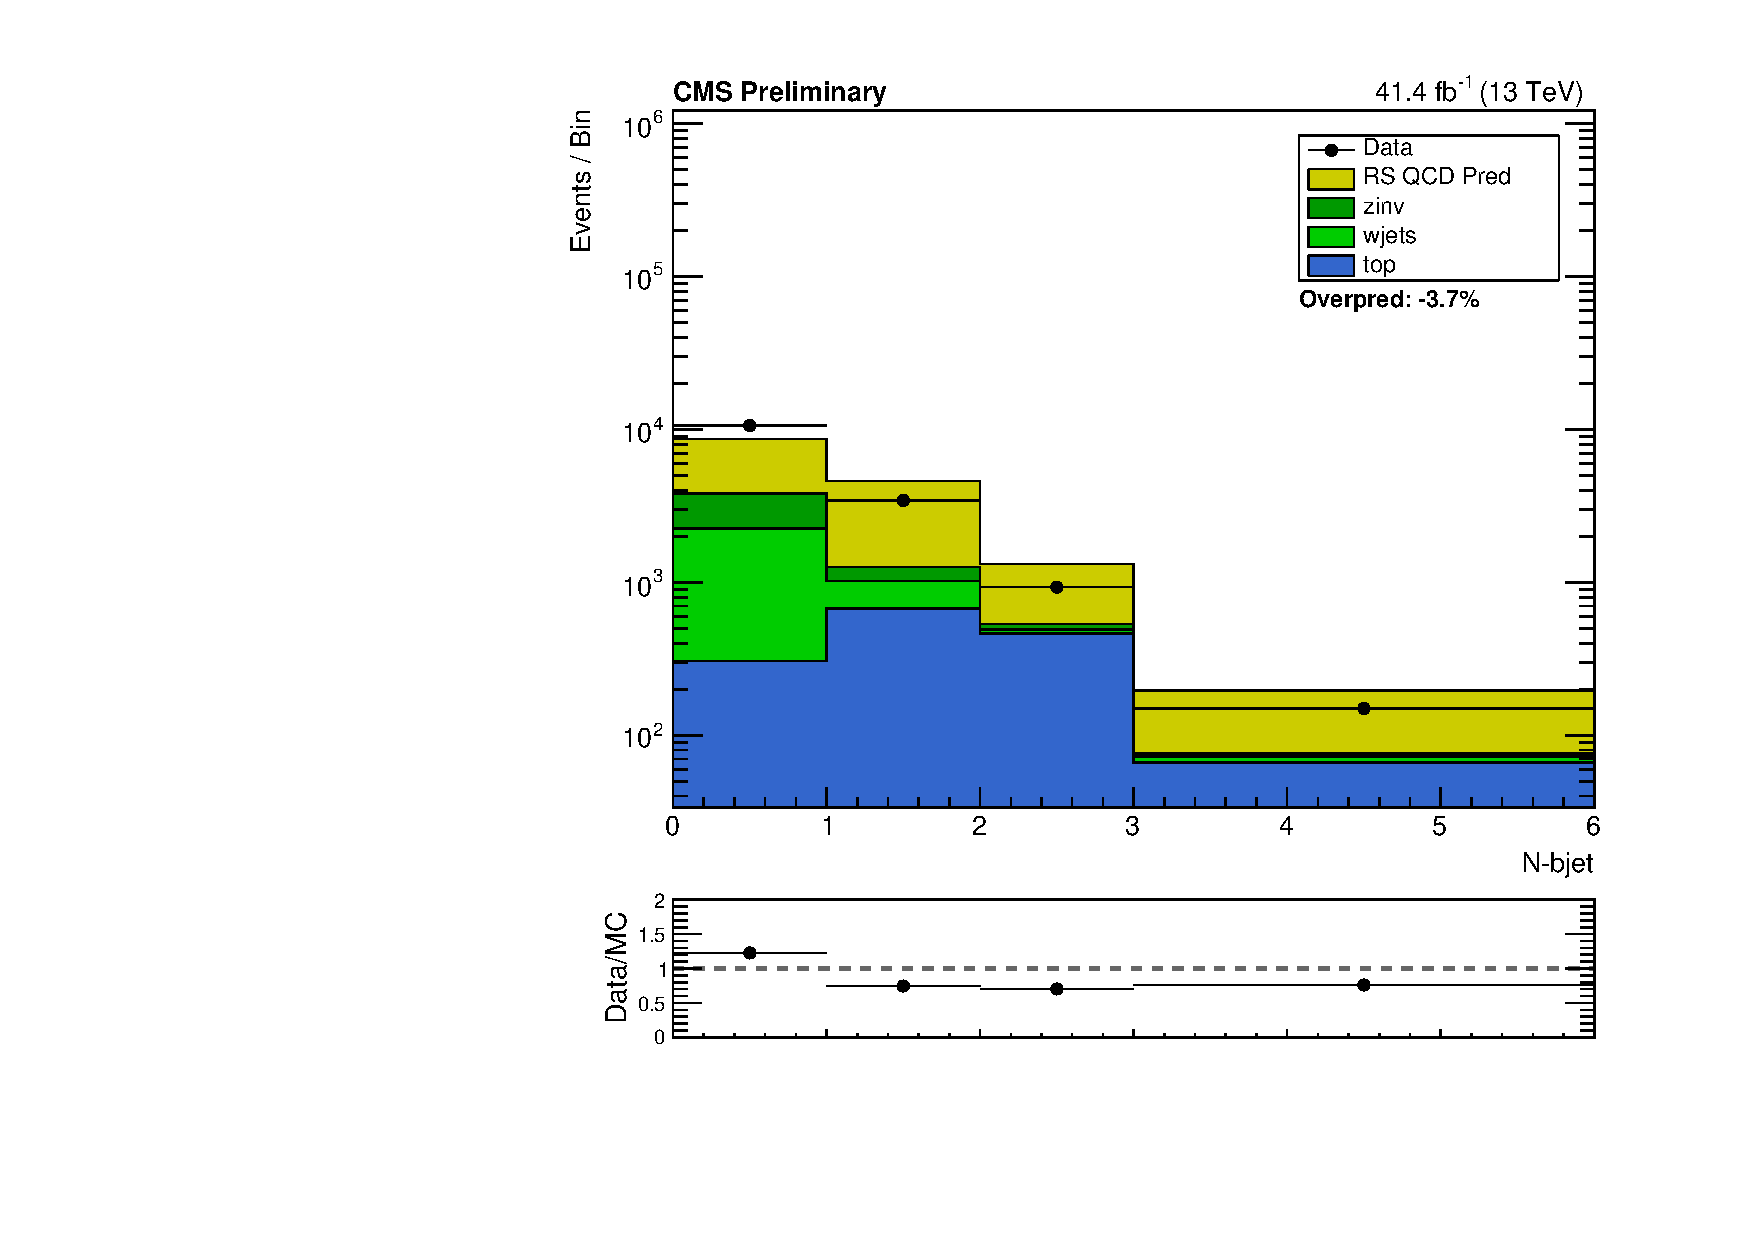
\includegraphics[width=0.49\textwidth]{figs/jetmet/nBJet20_DPhiMT2InclusiveHT450to1200_RecoBJet.pdf}
    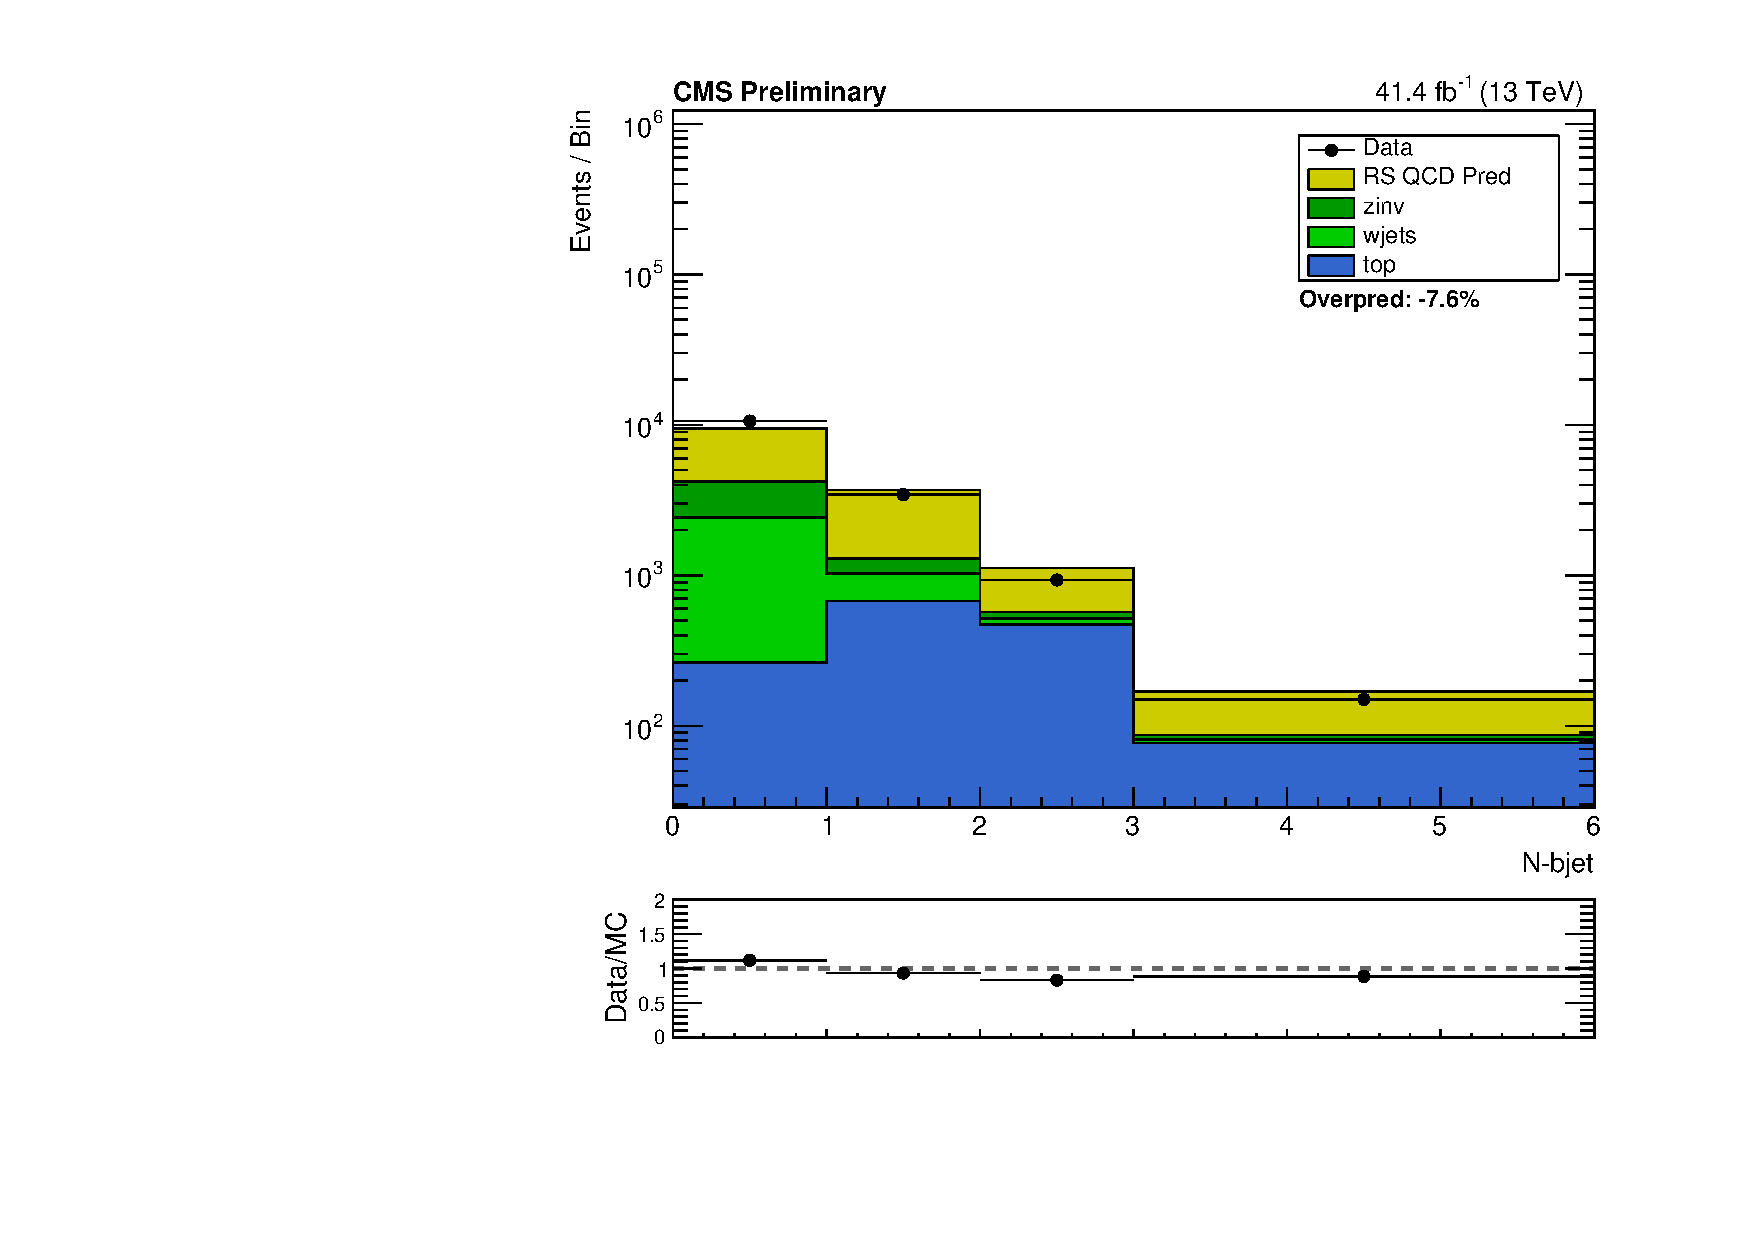
\includegraphics[width=0.49\textwidth]{figs/jetmet/nBJet20_DPhiMT2InclusiveHT450to1200_BTagSFs.pdf}
    \caption{The \nbtags distributions in the inverted-\dpmin + \mttwo sideband control region for $450 \leq \Ht < 1200$ GeV
    (described in Chapter~\ref{chap:qcd}),
    when (left) filling a single template based on reco jet medium b tagging, and (right) filling both histograms with
    weights given by the corrected probability of tagging a given jet as a medium b jet. Observed data are shown
    as black points, and prediction from the full Rebalance and Smear method is shown in yellow.
    Significant improvement is seen when using the second method. Residual shape discrepancies are 
    covered by a dedicated \nbtags shape systematic in the final estimate.
    }
    \label{fig:jrt_nb}
  \end{center}
\end{figure}


\subsection{Fits and jet energy resolution corrections}
\label{sec:jrt_fits}

Once the templates are derived, it is useful to split each template into a gaussian ``core'' and
non-gaussian ``tails'' The reason for this is twofold. First, it is known that jet resolution
is slightly different in data than in MC. This only applies to the standard gaussian smearing of the jets,
so in order to correct for the differences the gaussian core must be isolated.
Second, is is useful for studies on systematics to be able to alter the core/tails of the
templates individually. For example, to study the effect of mis-modeling in the tails,
one should be able to modify the size of the tails without affecting the size/shape
of the gaussian core.

To fit the core of a template, a gaussian is fitted in the range (mean $\pm$ RMS), where mean and RMS
are the mean and standard deviation of the template.
When measuring jet energy resolution and deriving scale factors, CMS only defines the core
of the jet response function as extending out to $\pm2\sigma$ of the fitted gaussian~\cite{JME_jes_jer}.
To be consistent, we use the same definition here, and in order to avoid discontinuities,
we linearly scale the gaussian to 0 between $\pm1$ and 2 $\sigma$. Precisely, if $g(x)$ is the
full fitted gaussian, and $\mu$ and $\sigma$ are its mean and standard deviation, our defined core function is
\[
\text{Core}(x) = 
\begin{cases}
g(x) & \text{if } |x-\mu| \leq 1\sigma \\
g(x)\left(2-\frac{|x-\mu|}{\sigma}\right) & \text{if } 1\sigma < |x-\mu| \leq 2\sigma \\
0 & \text{if } |x-\mu| > 2\sigma \\
\end{cases}.
\]

The tails are then simply defined as the full template function minus $\text{Core}(x)$.
Examples of this fitting procedure are shown in Fig.~\ref{fig:jrt_examples}. The truncated-gaussian
cores are shown in red, and the tails in green.

The first way that these fits are used is in the correction of the templates for jet energy resolution
differences between data and MC. The JetMET group provides year-dependent scale factors binned in 
$\eta$, shown in Table~\ref{tab:jrt_jersfs}. When smearing data events, the core of the template for a given jet
is widened by this scale factor before drawing a random smear factor from the distribution. This is done in a 
way to preserve the relative core/tail normalization. Specifically, if $\alpha$ is the scale factor by which we
want to widen the core, the modified template is given by
\[
f_\alpha(x) = \frac{1}{\alpha}\cdot\text{Core}((x-1)/\alpha+1) + \text{Tail}(x).
\]

\begin{table}[htp]
\caption{Jet energy resolution scale factors (data resolution divided by MC resolution) provided by the JetMET group.
             Uncertainties are statistical plus systematic.}
\label{tab:jrt_jersfs}
\centering
%\small
\begin{tabular}{|c|ccc|}
\hline
 & 2016 & 2017 & 2018 \\ \hline
$0.0 \leq |\eta| < 0.5$ & $1.160\pm0.065$ & $1.143\pm0.022$ & $1.150\pm0.042$ \\
$0.5 \leq |\eta| < 0.8$ & $1.195\pm0.065$ & $1.182\pm0.048$ & $1.134\pm0.080$ \\
$0.8 \leq |\eta| < 1.1$ & $1.146\pm0.063$ & $1.099\pm0.046$ & $1.102\pm0.052$ \\
$1.1 \leq |\eta| < 1.3$ & $1.161\pm0.103$ & $1.114\pm0.140$ & $1.134\pm0.112$ \\
$1.3 \leq |\eta| < 1.7$ & $1.128\pm0.099$ & $1.131\pm0.147$ & $1.104\pm0.211$ \\
$1.7 \leq |\eta| < 1.9$ & $1.100\pm0.108$ & $1.160\pm0.097$ & $1.149\pm0.159$ \\
$1.9 \leq |\eta| < 2.1$ & $1.143\pm0.121$ & $1.239\pm0.191$ & $1.148\pm0.209$ \\
$2.1 \leq |\eta| < 2.3$ & $1.151\pm0.114$ & $1.260\pm0.150$ & $1.114\pm0.191$ \\
$2.3 \leq |\eta| < 2.5$ & $1.296\pm0.237$ & $1.409\pm0.202$ & $1.347\pm0.274$ \\
$2.5 \leq |\eta| < 2.8$ & $1.342\pm0.209$ & $1.991\pm0.568$ & $2.137\pm0.524$ \\
$2.8 \leq |\eta| < 3.0$ & $1.779\pm0.201$ & $2.292\pm0.374$ & $1.650\pm0.941$ \\
$3.0 \leq |\eta| < 3.2$ & $1.187\pm0.124$ & $1.270\pm0.109$ & $1.225\pm0.194$ \\
$|\eta| \geq 3.2$       & $1.192\pm0.149$ & $1.154\pm0.152$ & $1.082\pm0.198$ \\
\hline
\end{tabular}
\end{table}

To assign a systematic from uncertainty in the jet energy resolution modeling, the smearing is run three times:
once using the central values in Table~\ref{tab:jrt_jersfs}, once with the $+1\sigma$ values,
and once with the $-1\sigma$ values. The differences in final signal region predictions,
integrated over each \Ht region, are used to assign a systematic uncertainty. The results of this
procedure are shown in Fig.~\ref{Fig:rs_data_JER_var} in Sec.~\ref{sec:rs_jrt_core}.

The fitted tails are used in a similar way to assign a systematic due to uncertainty in the tail modeling.
The tails are not stretched along the $x$ direction, but instead simply scaled up/down (i.e., their normalization
relative to the core is increased/decreased). Formally, to increase the tail size by a factor $\beta$, the
modified template is given by
\[
   f_\beta(x) = N_\beta(\text{Core}(x) + \beta\cdot\text{Tail}(x)),
\]
where $N_\beta$ is a normalization factor to ensure that the template integral remains equal to one.
Results of applying this procedure to the smearing of QCD MC with $\beta=1.25$ and 1.50 
are shown in Fig.~\ref{Fig:rs_modify_tail} in Sec.~\ref{sec:rs_jrt_tail}. 
The differences in final signal region yields with $\beta=1.25$ are used to assign a systematic uncertainty.
